% PREAMBLE
\documentclass[11pt]{amsart}
\usepackage[T1]{fontenc}
\usepackage{lmodern}
\usepackage{microtype}
\usepackage{amsmath,amssymb}
\usepackage{mathtools}
\usepackage{graphicx}
\usepackage{booktabs}
\usepackage{tikz}
\usepackage[colorlinks=true,linkcolor=blue!45!black,citecolor=blue!45!black,urlcolor=blue!45!black]{hyperref}
\usepackage[capitalize]{cleveref}

\newtheorem{theorem}{Theorem}[section]
\newtheorem{proposition}[theorem]{Proposition}
\newtheorem{lemma}[theorem]{Lemma}
\newtheorem{corollary}[theorem]{Corollary}
\newtheorem{conjecture}[theorem]{Conjecture}
\theoremstyle{definition}
\newtheorem{definition}[theorem]{Definition}
\newtheorem{fact}[theorem]{Fact}
\theoremstyle{remark}
\newtheorem{remark}[theorem]{Remark}

\title{The First Base Below a Quarter}
\author{Carlo Mitchener}
\address{MrlyProd, Inc.}
\email{carlo.mitchener@gmail.com}
\date{First published 2026-09-07}

% PAPER
\begin{document}

\begin{abstract}
Drop one digit from a base and look at the numbers you can still write. How much of the Fourier mass of that set survives is measured by a single number, its $\ell^1$ exponent, and a sieve turns on when the number falls below a quarter. This paper locates the threshold. Base $21$ with the digit $0$ removed is the first base carrying any such set below a quarter; base $34$ is the first base whose every excluded digit clears; and a bound that names the base and forgets the digit proves clearance for every base from $126$ up, so the family floor $34$ is exact.
\end{abstract}

% TITLE PAGE
\makeatletter
\global\let\titledate\@date
\global\let\paperabstract\@setabstracta
\global\let\@date\@empty
\global\let\@setabstract\relax
\makeatother

\maketitle

\begin{center}
\normalfont\footnotesize\titledate
\end{center}

\vspace*{\stretch{1}}

\begin{center}

\includegraphics[width=0.5\textwidth]{figures/avatar.png}
\end{center}

\vspace*{\stretch{1.25}}

\newpage

\paperabstract

% BODY
\emergencystretch=2em

\section{Introduction}
\label{sec:intro}

Fix a base $q$ and cross out one digit. What is left is a set of integers: those you can still write, the ones whose base-$q$ expansion never uses the missing digit. In base $10$ with the digit $7$ removed these are $1, 2, \dots, 6, 8, 9, 10, \dots, 69, 80, \dots$, and there are $9^{L}$ of them below $10^{L}$, so the set is thin but not very thin. Sets of this shape are the standard test bed for analytic number theory on a fractal: Maynard proved that infinitely many of them are prime in base $10$ \cite{may}, and everything in that proof passes through the set by way of its Fourier transform.

The transform is one function on the circle. Write
\[
  \widehat{F}(t) \;=\; \frac{1}{q-1}\sum_{\substack{0 \le a < q \\ a \ne a_{0}}} e(a t), \qquad e(x) = e^{2\pi i x},
\]
for the normalised character sum of the surviving digits $F = \{0, \dots, q-1\} \setminus \{a_{0}\}$, and $\widehat{F}_{L}(t) = \prod_{j<L} \widehat{F}(q^{j} t)$ for the transform of the $L$-digit strings. A sieve does not read $\widehat{F}_{L}$ pointwise; it reads how much of it survives when the whole grid of $q^{L}$ frequencies is added up in absolute value. The growth rate of that grid sum is one number, the \emph{$\ell^{1}$ exponent} $\alpha_{1}$ of \cref{def:alpha}, and it is the number this paper is about. Small $\alpha_{1}$ means the digit restriction cancels; $\alpha_{1}$ close to $1$ means it barely does.

\begin{figure}[t]
\centering
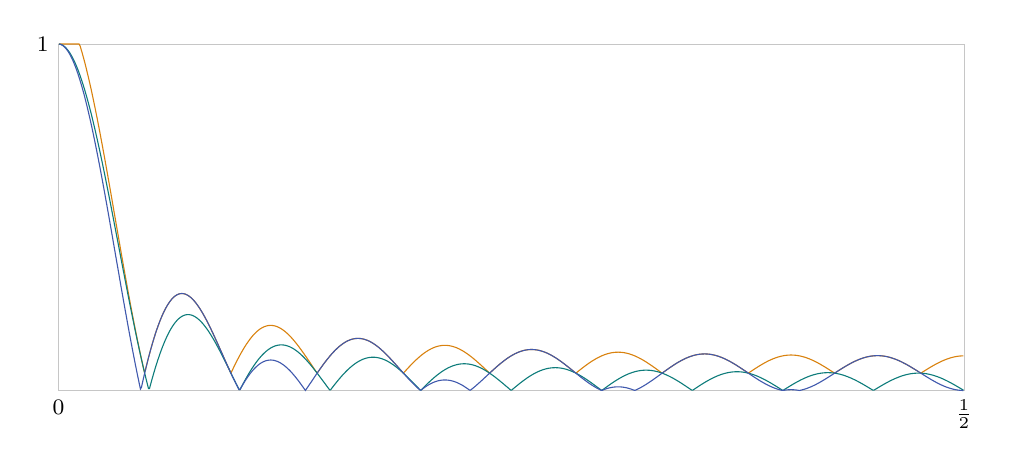
\begin{tikzpicture}[x=23cm,y=4.4cm]
\definecolor{tonebound}{HTML}{D9820F}
\definecolor{tonegasket}{HTML}{0E7C7B}
\definecolor{tonecarpet}{HTML}{4059AD}
\draw[gray!45,line width=0.3pt] (0,0) rectangle (0.5,1);
\draw[tonebound,line width=0.4pt] plot coordinates {(0.00028,1.00000) (0.00083,1.00000) (0.00139,1.00000) (0.00194,1.00000) (0.00250,1.00000) (0.00306,1.00000) (0.00361,1.00000) (0.00417,1.00000) (0.00472,1.00000) (0.00528,1.00000) (0.00583,1.00000) (0.00639,1.00000) (0.00694,1.00000) (0.00750,1.00000) (0.00806,1.00000) (0.00861,1.00000) (0.00917,1.00000) (0.00972,1.00000) (0.01028,1.00000) (0.01083,1.00000) (0.01139,1.00000) (0.01194,0.99488) (0.01250,0.98521) (0.01306,0.97516) (0.01361,0.96475) (0.01417,0.95397) (0.01472,0.94284) (0.01528,0.93137) (0.01583,0.91956) (0.01639,0.90742) (0.01694,0.89497) (0.01750,0.88221) (0.01806,0.86916) (0.01861,0.85582) (0.01917,0.84220) (0.01972,0.82832) (0.02028,0.81418) (0.02083,0.79980) (0.02139,0.78519) (0.02194,0.77035) (0.02250,0.75530) (0.02306,0.74006) (0.02361,0.72463) (0.02417,0.70902) (0.02472,0.69325) (0.02528,0.67733) (0.02583,0.66127) (0.02639,0.64508) (0.02694,0.62878) (0.02750,0.61238) (0.02806,0.59588) (0.02861,0.57930) (0.02917,0.56266) (0.02972,0.54597) (0.03028,0.52923) (0.03083,0.51247) (0.03139,0.49568) (0.03194,0.47890) (0.03250,0.46212) (0.03306,0.44535) (0.03361,0.42862) (0.03417,0.41194) (0.03472,0.39530) (0.03528,0.37874) (0.03583,0.36225) (0.03639,0.34585) (0.03694,0.32955) (0.03750,0.31336) (0.03806,0.29730) (0.03861,0.28136) (0.03917,0.26558) (0.03972,0.24994) (0.04028,0.23448) (0.04083,0.21918) (0.04139,0.20407) (0.04194,0.18916) (0.04250,0.17445) (0.04306,0.15995) (0.04361,0.14568) (0.04417,0.13163) (0.04472,0.11782) (0.04528,0.10426) (0.04583,0.09096) (0.04639,0.07791) (0.04694,0.06514) (0.04750,0.05264) (0.04806,0.05957) (0.04861,0.07150) (0.04917,0.08313) (0.04972,0.09445) (0.05028,0.10547) (0.05083,0.11618) (0.05139,0.12657) (0.05194,0.13664) (0.05250,0.14638) (0.05306,0.15579) (0.05361,0.16487) (0.05417,0.17361) (0.05472,0.18201) (0.05528,0.19007) (0.05583,0.19778) (0.05639,0.20515) (0.05694,0.21217) (0.05750,0.21884) (0.05806,0.22516) (0.05861,0.23113) (0.05917,0.23675) (0.05972,0.24201) (0.06028,0.24693) (0.06083,0.25149) (0.06139,0.25571) (0.06194,0.25958) (0.06250,0.26310) (0.06306,0.26628) (0.06361,0.26911) (0.06417,0.27161) (0.06472,0.27376) (0.06528,0.27559) (0.06583,0.27709) (0.06639,0.27825) (0.06694,0.27910) (0.06750,0.27963) (0.06806,0.27984) (0.06861,0.27975) (0.06917,0.27935) (0.06972,0.27865) (0.07028,0.27766) (0.07083,0.27638) (0.07139,0.27482) (0.07194,0.27298) (0.07250,0.27088) (0.07306,0.26851) (0.07361,0.26589) (0.07417,0.26302) (0.07472,0.25991) (0.07528,0.25656) (0.07583,0.25299) (0.07639,0.24920) (0.07694,0.24519) (0.07750,0.24099) (0.07806,0.23658) (0.07861,0.23200) (0.07917,0.22723) (0.07972,0.22229) (0.08028,0.21718) (0.08083,0.21193) (0.08139,0.20653) (0.08194,0.20099) (0.08250,0.19532) (0.08306,0.18954) (0.08361,0.18364) (0.08417,0.17764) (0.08472,0.17155) (0.08528,0.16538) (0.08583,0.15913) (0.08639,0.15281) (0.08694,0.14643) (0.08750,0.14001) (0.08806,0.13354) (0.08861,0.12704) (0.08917,0.12052) (0.08972,0.11398) (0.09028,0.10743) (0.09083,0.10089) (0.09139,0.09436) (0.09194,0.08784) (0.09250,0.08135) (0.09306,0.07489) (0.09361,0.06848) (0.09417,0.06211) (0.09472,0.05580) (0.09528,0.05044) (0.09583,0.05662) (0.09639,0.06272) (0.09694,0.06873) (0.09750,0.07465) (0.09806,0.08048) (0.09861,0.08620) (0.09917,0.09181) (0.09972,0.09730) (0.10028,0.10267) (0.10083,0.10791) (0.10139,0.11303) (0.10194,0.11800) (0.10250,0.12283) (0.10306,0.12751) (0.10361,0.13204) (0.10417,0.13642) (0.10472,0.14063) (0.10528,0.14469) (0.10583,0.14857) (0.10639,0.15228) (0.10694,0.15583) (0.10750,0.15919) (0.10806,0.16237) (0.10861,0.16538) (0.10917,0.16820) (0.10972,0.17083) (0.11028,0.17328) (0.11083,0.17554) (0.11139,0.17762) (0.11194,0.17950) (0.11250,0.18119) (0.11306,0.18269) (0.11361,0.18400) (0.11417,0.18512) (0.11472,0.18605) (0.11528,0.18678) (0.11583,0.18733) (0.11639,0.18769) (0.11694,0.18787) (0.11750,0.18786) (0.11806,0.18766) (0.11861,0.18728) (0.11917,0.18672) (0.11972,0.18599) (0.12028,0.18508) (0.12083,0.18400) (0.12139,0.18274) (0.12194,0.18133) (0.12250,0.17975) (0.12306,0.17801) (0.12361,0.17611) (0.12417,0.17406) (0.12472,0.17186) (0.12528,0.16952) (0.12583,0.16704) (0.12639,0.16442) (0.12694,0.16168) (0.12750,0.15880) (0.12806,0.15581) (0.12861,0.15270) (0.12917,0.14947) (0.12972,0.14614) (0.13028,0.14271) (0.13083,0.13918) (0.13139,0.13556) (0.13194,0.13186) (0.13250,0.12807) (0.13306,0.12421) (0.13361,0.12028) (0.13417,0.11629) (0.13472,0.11224) (0.13528,0.10814) (0.13583,0.10400) (0.13639,0.09981) (0.13694,0.09559) (0.13750,0.09134) (0.13806,0.08706) (0.13861,0.08277) (0.13917,0.07847) (0.13972,0.07416) (0.14028,0.06985) (0.14083,0.06555) (0.14139,0.06125) (0.14194,0.05698) (0.14250,0.05272) (0.14306,0.05151) (0.14361,0.05570) (0.14417,0.05986) (0.14472,0.06397) (0.14528,0.06804) (0.14583,0.07205) (0.14639,0.07601) (0.14694,0.07990) (0.14750,0.08373) (0.14806,0.08749) (0.14861,0.09116) (0.14917,0.09476) (0.14972,0.09828) (0.15028,0.10170) (0.15083,0.10503) (0.15139,0.10827) (0.15194,0.11141) (0.15250,0.11444) (0.15306,0.11737) (0.15361,0.12019) (0.15417,0.12289) (0.15472,0.12548) (0.15528,0.12796) (0.15583,0.13031) (0.15639,0.13254) (0.15694,0.13464) (0.15750,0.13662) (0.15806,0.13847) (0.15861,0.14019) (0.15917,0.14178) (0.15972,0.14323) (0.16028,0.14455) (0.16083,0.14574) (0.16139,0.14679) (0.16194,0.14771) (0.16250,0.14849) (0.16306,0.14913) (0.16361,0.14964) (0.16417,0.15001) (0.16472,0.15024) (0.16528,0.15034) (0.16583,0.15030) (0.16639,0.15013) (0.16694,0.14983) (0.16750,0.14940) (0.16806,0.14883) (0.16861,0.14814) (0.16917,0.14732) (0.16972,0.14638) (0.17028,0.14531) (0.17083,0.14412) (0.17139,0.14281) (0.17194,0.14139) (0.17250,0.13985) (0.17306,0.13820) (0.17361,0.13644) (0.17417,0.13458) (0.17472,0.13261) (0.17528,0.13055) (0.17583,0.12839) (0.17639,0.12613) (0.17694,0.12379) (0.17750,0.12136) (0.17806,0.11885) (0.17861,0.11627) (0.17917,0.11360) (0.17972,0.11087) (0.18028,0.10807) (0.18083,0.10521) (0.18139,0.10229) (0.18194,0.09932) (0.18250,0.09630) (0.18306,0.09323) (0.18361,0.09012) (0.18417,0.08697) (0.18472,0.08379) (0.18528,0.08058) (0.18583,0.07735) (0.18639,0.07410) (0.18694,0.07083) (0.18750,0.06756) (0.18806,0.06427) (0.18861,0.06099) (0.18917,0.05771) (0.18972,0.05443) (0.19028,0.05116) (0.19083,0.05209) (0.19139,0.05532) (0.19194,0.05853) (0.19250,0.06171) (0.19306,0.06486) (0.19361,0.06797) (0.19417,0.07104) (0.19472,0.07407) (0.19528,0.07705) (0.19583,0.07999) (0.19639,0.08286) (0.19694,0.08568) (0.19750,0.08844) (0.19806,0.09113) (0.19861,0.09376) (0.19917,0.09631) (0.19972,0.09879) (0.20028,0.10119) (0.20083,0.10351) (0.20139,0.10575) (0.20194,0.10791) (0.20250,0.10997) (0.20306,0.11195) (0.20361,0.11384) (0.20417,0.11563) (0.20472,0.11732) (0.20528,0.11892) (0.20583,0.12041) (0.20639,0.12181) (0.20694,0.12310) (0.20750,0.12429) (0.20806,0.12538) (0.20861,0.12636) (0.20917,0.12723) (0.20972,0.12800) (0.21028,0.12865) (0.21083,0.12920) (0.21139,0.12965) (0.21194,0.12998) (0.21250,0.13020) (0.21306,0.13032) (0.21361,0.13033) (0.21417,0.13023) (0.21472,0.13002) (0.21528,0.12971) (0.21583,0.12929) (0.21639,0.12877) (0.21694,0.12815) (0.21750,0.12742) (0.21806,0.12659) (0.21861,0.12567) (0.21917,0.12465) (0.21972,0.12353) (0.22028,0.12231) (0.22083,0.12101) (0.22139,0.11962) (0.22194,0.11814) (0.22250,0.11657) (0.22306,0.11492) (0.22361,0.11320) (0.22417,0.11139) (0.22472,0.10951) (0.22528,0.10756) (0.22583,0.10554) (0.22639,0.10345) (0.22694,0.10130) (0.22750,0.09909) (0.22806,0.09682) (0.22861,0.09450) (0.22917,0.09213) (0.22972,0.08971) (0.23028,0.08725) (0.23083,0.08475) (0.23139,0.08221) (0.23194,0.07964) (0.23250,0.07704) (0.23306,0.07441) (0.23361,0.07176) (0.23417,0.06910) (0.23472,0.06641) (0.23528,0.06372) (0.23583,0.06101) (0.23639,0.05831) (0.23694,0.05560) (0.23750,0.05289) (0.23806,0.05019) (0.23861,0.05250) (0.23917,0.05517) (0.23972,0.05783) (0.24028,0.06047) (0.24083,0.06309) (0.24139,0.06567) (0.24194,0.06823) (0.24250,0.07076) (0.24306,0.07324) (0.24361,0.07569) (0.24417,0.07809) (0.24472,0.08045) (0.24528,0.08276) (0.24583,0.08501) (0.24639,0.08721) (0.24694,0.08936) (0.24750,0.09144) (0.24806,0.09346) (0.24861,0.09541) (0.24917,0.09730) (0.24972,0.09912) (0.25028,0.10086) (0.25083,0.10253) (0.25139,0.10413) (0.25194,0.10565) (0.25250,0.10708) (0.25306,0.10844) (0.25361,0.10971) (0.25417,0.11090) (0.25472,0.11201) (0.25528,0.11302) (0.25583,0.11395) (0.25639,0.11479) (0.25694,0.11554) (0.25750,0.11620) (0.25806,0.11677) (0.25861,0.11725) (0.25917,0.11764) (0.25972,0.11794) (0.26028,0.11814) (0.26083,0.11825) (0.26139,0.11827) (0.26194,0.11820) (0.26250,0.11804) (0.26306,0.11778) (0.26361,0.11744) (0.26417,0.11701) (0.26472,0.11649) (0.26528,0.11588) (0.26583,0.11519) (0.26639,0.11441) (0.26694,0.11355) (0.26750,0.11260) (0.26806,0.11158) (0.26861,0.11047) (0.26917,0.10929) (0.26972,0.10803) (0.27028,0.10670) (0.27083,0.10530) (0.27139,0.10382) (0.27194,0.10228) (0.27250,0.10068) (0.27306,0.09901) (0.27361,0.09728) (0.27417,0.09549) (0.27472,0.09365) (0.27528,0.09175) (0.27583,0.08980) (0.27639,0.08781) (0.27694,0.08577) (0.27750,0.08369) (0.27806,0.08157) (0.27861,0.07942) (0.27917,0.07723) (0.27972,0.07501) (0.28028,0.07276) (0.28083,0.07049) (0.28139,0.06820) (0.28194,0.06589) (0.28250,0.06357) (0.28306,0.06124) (0.28361,0.05889) (0.28417,0.05654) (0.28472,0.05419) (0.28528,0.05184) (0.28583,0.05050) (0.28639,0.05284) (0.28694,0.05517) (0.28750,0.05748) (0.28806,0.05978) (0.28861,0.06206) (0.28917,0.06432) (0.28972,0.06655) (0.29028,0.06875) (0.29083,0.07092) (0.29139,0.07306) (0.29194,0.07516) (0.29250,0.07723) (0.29306,0.07925) (0.29361,0.08122) (0.29417,0.08315) (0.29472,0.08503) (0.29528,0.08686) (0.29583,0.08863) (0.29639,0.09035) (0.29694,0.09201) (0.29750,0.09361) (0.29806,0.09514) (0.29861,0.09661) (0.29917,0.09802) (0.29972,0.09936) (0.30028,0.10063) (0.30083,0.10182) (0.30139,0.10295) (0.30194,0.10400) (0.30250,0.10497) (0.30306,0.10587) (0.30361,0.10670) (0.30417,0.10744) (0.30472,0.10811) (0.30528,0.10870) (0.30583,0.10920) (0.30639,0.10963) (0.30694,0.10997) (0.30750,0.11024) (0.30806,0.11042) (0.30861,0.11052) (0.30917,0.11054) (0.30972,0.11048) (0.31028,0.11034) (0.31083,0.11012) (0.31139,0.10982) (0.31194,0.10944) (0.31250,0.10898) (0.31306,0.10844) (0.31361,0.10783) (0.31417,0.10714) (0.31472,0.10637) (0.31528,0.10553) (0.31583,0.10462) (0.31639,0.10364) (0.31694,0.10259) (0.31750,0.10147) (0.31806,0.10028) (0.31861,0.09903) (0.31917,0.09771) (0.31972,0.09634) (0.32028,0.09490) (0.32083,0.09341) (0.32139,0.09187) (0.32194,0.09027) (0.32250,0.08862) (0.32306,0.08692) (0.32361,0.08518) (0.32417,0.08339) (0.32472,0.08157) (0.32528,0.07970) (0.32583,0.07780) (0.32639,0.07587) (0.32694,0.07390) (0.32750,0.07191) (0.32806,0.06989) (0.32861,0.06785) (0.32917,0.06579) (0.32972,0.06372) (0.33028,0.06162) (0.33083,0.05952) (0.33139,0.05741) (0.33194,0.05530) (0.33250,0.05318) (0.33306,0.05106) (0.33361,0.05106) (0.33417,0.05317) (0.33472,0.05527) (0.33528,0.05736) (0.33583,0.05944) (0.33639,0.06150) (0.33694,0.06354) (0.33750,0.06556) (0.33806,0.06755) (0.33861,0.06952) (0.33917,0.07145) (0.33972,0.07336) (0.34028,0.07522) (0.34083,0.07706) (0.34139,0.07885) (0.34194,0.08060) (0.34250,0.08230) (0.34306,0.08396) (0.34361,0.08557) (0.34417,0.08713) (0.34472,0.08864) (0.34528,0.09009) (0.34583,0.09149) (0.34639,0.09283) (0.34694,0.09410) (0.34750,0.09532) (0.34806,0.09648) (0.34861,0.09757) (0.34917,0.09859) (0.34972,0.09955) (0.35028,0.10044) (0.35083,0.10126) (0.35139,0.10201) (0.35194,0.10269) (0.35250,0.10329) (0.35306,0.10383) (0.35361,0.10429) (0.35417,0.10468) (0.35472,0.10499) (0.35528,0.10523) (0.35583,0.10540) (0.35639,0.10549) (0.35694,0.10551) (0.35750,0.10545) (0.35806,0.10532) (0.35861,0.10511) (0.35917,0.10484) (0.35972,0.10448) (0.36028,0.10406) (0.36083,0.10356) (0.36139,0.10300) (0.36194,0.10236) (0.36250,0.10165) (0.36306,0.10088) (0.36361,0.10004) (0.36417,0.09913) (0.36472,0.09816) (0.36528,0.09713) (0.36583,0.09603) (0.36639,0.09488) (0.36694,0.09367) (0.36750,0.09240) (0.36806,0.09107) (0.36861,0.08969) (0.36917,0.08826) (0.36972,0.08679) (0.37028,0.08526) (0.37083,0.08369) (0.37139,0.08208) (0.37194,0.08042) (0.37250,0.07873) (0.37306,0.07701) (0.37361,0.07524) (0.37417,0.07345) (0.37472,0.07163) (0.37528,0.06978) (0.37583,0.06791) (0.37639,0.06602) (0.37694,0.06411) (0.37750,0.06218) (0.37806,0.06024) (0.37861,0.05829) (0.37917,0.05633) (0.37972,0.05436) (0.38028,0.05239) (0.38083,0.05042) (0.38139,0.05155) (0.38194,0.05351) (0.38250,0.05546) (0.38306,0.05741) (0.38361,0.05934) (0.38417,0.06126) (0.38472,0.06316) (0.38528,0.06504) (0.38583,0.06690) (0.38639,0.06873) (0.38694,0.07054) (0.38750,0.07231) (0.38806,0.07406) (0.38861,0.07576) (0.38917,0.07744) (0.38972,0.07907) (0.39028,0.08066) (0.39083,0.08221) (0.39139,0.08371) (0.39194,0.08517) (0.39250,0.08658) (0.39306,0.08794) (0.39361,0.08924) (0.39417,0.09049) (0.39472,0.09169) (0.39528,0.09282) (0.39583,0.09390) (0.39639,0.09492) (0.39694,0.09588) (0.39750,0.09677) (0.39806,0.09761) (0.39861,0.09837) (0.39917,0.09907) (0.39972,0.09971) (0.40028,0.10028) (0.40083,0.10077) (0.40139,0.10120) (0.40194,0.10157) (0.40250,0.10186) (0.40306,0.10208) (0.40361,0.10223) (0.40417,0.10231) (0.40472,0.10233) (0.40528,0.10227) (0.40583,0.10214) (0.40639,0.10194) (0.40694,0.10168) (0.40750,0.10134) (0.40806,0.10093) (0.40861,0.10046) (0.40917,0.09992) (0.40972,0.09932) (0.41028,0.09865) (0.41083,0.09791) (0.41139,0.09711) (0.41194,0.09625) (0.41250,0.09533) (0.41306,0.09434) (0.41361,0.09330) (0.41417,0.09221) (0.41472,0.09105) (0.41528,0.08985) (0.41583,0.08859) (0.41639,0.08728) (0.41694,0.08592) (0.41750,0.08451) (0.41806,0.08306) (0.41861,0.08157) (0.41917,0.08003) (0.41972,0.07846) (0.42028,0.07685) (0.42083,0.07521) (0.42139,0.07353) (0.42194,0.07182) (0.42250,0.07009) (0.42306,0.06833) (0.42361,0.06655) (0.42417,0.06474) (0.42472,0.06292) (0.42528,0.06108) (0.42583,0.05923) (0.42639,0.05737) (0.42694,0.05550) (0.42750,0.05362) (0.42806,0.05175) (0.42861,0.05013) (0.42917,0.05201) (0.42972,0.05389) (0.43028,0.05575) (0.43083,0.05761) (0.43139,0.05946) (0.43194,0.06129) (0.43250,0.06311) (0.43306,0.06491) (0.43361,0.06668) (0.43417,0.06843) (0.43472,0.07016) (0.43528,0.07186) (0.43583,0.07353) (0.43639,0.07516) (0.43694,0.07676) (0.43750,0.07832) (0.43806,0.07985) (0.43861,0.08133) (0.43917,0.08277) (0.43972,0.08416) (0.44028,0.08551) (0.44083,0.08681) (0.44139,0.08806) (0.44194,0.08926) (0.44250,0.09040) (0.44306,0.09149) (0.44361,0.09253) (0.44417,0.09350) (0.44472,0.09442) (0.44528,0.09528) (0.44583,0.09607) (0.44639,0.09681) (0.44694,0.09748) (0.44750,0.09808) (0.44806,0.09862) (0.44861,0.09910) (0.44917,0.09951) (0.44972,0.09985) (0.45028,0.10013) (0.45083,0.10034) (0.45139,0.10048) (0.45194,0.10055) (0.45250,0.10056) (0.45306,0.10050) (0.45361,0.10037) (0.45417,0.10017) (0.45472,0.09991) (0.45528,0.09958) (0.45583,0.09918) (0.45639,0.09872) (0.45694,0.09819) (0.45750,0.09760) (0.45806,0.09694) (0.45861,0.09623) (0.45917,0.09545) (0.45972,0.09461) (0.46028,0.09371) (0.46083,0.09275) (0.46139,0.09173) (0.46194,0.09066) (0.46250,0.08954) (0.46306,0.08836) (0.46361,0.08714) (0.46417,0.08586) (0.46472,0.08453) (0.46528,0.08316) (0.46583,0.08175) (0.46639,0.08029) (0.46694,0.07880) (0.46750,0.07726) (0.46806,0.07569) (0.46861,0.07409) (0.46917,0.07245) (0.46972,0.07079) (0.47028,0.06910) (0.47083,0.06738) (0.47139,0.06564) (0.47194,0.06388) (0.47250,0.06210) (0.47306,0.06030) (0.47361,0.05850) (0.47417,0.05668) (0.47472,0.05485) (0.47528,0.05302) (0.47583,0.05118) (0.47639,0.05066) (0.47694,0.05249) (0.47750,0.05433) (0.47806,0.05615) (0.47861,0.05797) (0.47917,0.05978) (0.47972,0.06157) (0.48028,0.06335) (0.48083,0.06510) (0.48139,0.06684) (0.48194,0.06856) (0.48250,0.07025) (0.48306,0.07191) (0.48361,0.07354) (0.48417,0.07514) (0.48472,0.07671) (0.48528,0.07824) (0.48583,0.07974) (0.48639,0.08119) (0.48694,0.08260) (0.48750,0.08397) (0.48806,0.08529) (0.48861,0.08656) (0.48917,0.08779) (0.48972,0.08896) (0.49028,0.09008) (0.49083,0.09115) (0.49139,0.09216) (0.49194,0.09312) (0.49250,0.09402) (0.49306,0.09485) (0.49361,0.09563) (0.49417,0.09635) (0.49472,0.09701) (0.49528,0.09760) (0.49583,0.09813) (0.49639,0.09859) (0.49694,0.09899) (0.49750,0.09932) (0.49806,0.09959) (0.49861,0.09979) (0.49917,0.09992) (0.49972,0.09999)};
\draw[tonegasket,line width=0.4pt] plot coordinates {(0.00028,0.99995) (0.00083,0.99954) (0.00139,0.99873) (0.00194,0.99752) (0.00250,0.99590) (0.00306,0.99388) (0.00361,0.99146) (0.00417,0.98864) (0.00472,0.98543) (0.00528,0.98182) (0.00583,0.97782) (0.00639,0.97342) (0.00694,0.96865) (0.00750,0.96349) (0.00806,0.95795) (0.00861,0.95204) (0.00917,0.94575) (0.00972,0.93910) (0.01028,0.93209) (0.01083,0.92473) (0.01139,0.91701) (0.01194,0.90895) (0.01250,0.90055) (0.01306,0.89181) (0.01361,0.88275) (0.01417,0.87337) (0.01472,0.86367) (0.01528,0.85367) (0.01583,0.84337) (0.01639,0.83278) (0.01694,0.82190) (0.01750,0.81074) (0.01806,0.79931) (0.01861,0.78763) (0.01917,0.77569) (0.01972,0.76351) (0.02028,0.75109) (0.02083,0.73844) (0.02139,0.72558) (0.02194,0.71250) (0.02250,0.69923) (0.02306,0.68576) (0.02361,0.67212) (0.02417,0.65830) (0.02472,0.64432) (0.02528,0.63019) (0.02583,0.61592) (0.02639,0.60151) (0.02694,0.58698) (0.02750,0.57233) (0.02806,0.55758) (0.02861,0.54274) (0.02917,0.52782) (0.02972,0.51282) (0.03028,0.49776) (0.03083,0.48265) (0.03139,0.46749) (0.03194,0.45230) (0.03250,0.43709) (0.03306,0.42187) (0.03361,0.40664) (0.03417,0.39142) (0.03472,0.37622) (0.03528,0.36104) (0.03583,0.34590) (0.03639,0.33081) (0.03694,0.31577) (0.03750,0.30080) (0.03806,0.28590) (0.03861,0.27109) (0.03917,0.25637) (0.03972,0.24176) (0.04028,0.22725) (0.04083,0.21287) (0.04139,0.19861) (0.04194,0.18449) (0.04250,0.17052) (0.04306,0.15670) (0.04361,0.14304) (0.04417,0.12955) (0.04472,0.11624) (0.04528,0.10312) (0.04583,0.09019) (0.04639,0.07745) (0.04694,0.06492) (0.04750,0.05261) (0.04806,0.04052) (0.04861,0.02865) (0.04917,0.01701) (0.04972,0.00561) (0.05028,0.00555) (0.05083,0.01646) (0.05139,0.02711) (0.05194,0.03751) (0.05250,0.04764) (0.05306,0.05750) (0.05361,0.06710) (0.05417,0.07642) (0.05472,0.08545) (0.05528,0.09421) (0.05583,0.10268) (0.05639,0.11086) (0.05694,0.11875) (0.05750,0.12635) (0.05806,0.13365) (0.05861,0.14065) (0.05917,0.14735) (0.05972,0.15375) (0.06028,0.15985) (0.06083,0.16565) (0.06139,0.17115) (0.06194,0.17634) (0.06250,0.18123) (0.06306,0.18581) (0.06361,0.19009) (0.06417,0.19407) (0.06472,0.19775) (0.06528,0.20113) (0.06583,0.20420) (0.06639,0.20699) (0.06694,0.20947) (0.06750,0.21167) (0.06806,0.21357) (0.06861,0.21519) (0.06917,0.21652) (0.06972,0.21757) (0.07028,0.21834) (0.07083,0.21883) (0.07139,0.21906) (0.07194,0.21901) (0.07250,0.21871) (0.07306,0.21814) (0.07361,0.21732) (0.07417,0.21625) (0.07472,0.21493) (0.07528,0.21337) (0.07583,0.21158) (0.07639,0.20956) (0.07694,0.20732) (0.07750,0.20485) (0.07806,0.20217) (0.07861,0.19929) (0.07917,0.19620) (0.07972,0.19292) (0.08028,0.18946) (0.08083,0.18581) (0.08139,0.18198) (0.08194,0.17799) (0.08250,0.17383) (0.08306,0.16952) (0.08361,0.16505) (0.08417,0.16045) (0.08472,0.15571) (0.08528,0.15085) (0.08583,0.14586) (0.08639,0.14076) (0.08694,0.13556) (0.08750,0.13025) (0.08806,0.12485) (0.08861,0.11937) (0.08917,0.11381) (0.08972,0.10818) (0.09028,0.10249) (0.09083,0.09674) (0.09139,0.09094) (0.09194,0.08510) (0.09250,0.07922) (0.09306,0.07332) (0.09361,0.06740) (0.09417,0.06146) (0.09472,0.05552) (0.09528,0.04958) (0.09583,0.04364) (0.09639,0.03772) (0.09694,0.03181) (0.09750,0.02594) (0.09806,0.02010) (0.09861,0.01429) (0.09917,0.00854) (0.09972,0.00283) (0.10028,0.00282) (0.10083,0.00840) (0.10139,0.01392) (0.10194,0.01936) (0.10250,0.02471) (0.10306,0.02999) (0.10361,0.03517) (0.10417,0.04026) (0.10472,0.04525) (0.10528,0.05013) (0.10583,0.05490) (0.10639,0.05955) (0.10694,0.06409) (0.10750,0.06851) (0.10806,0.07280) (0.10861,0.07696) (0.10917,0.08098) (0.10972,0.08487) (0.11028,0.08862) (0.11083,0.09222) (0.11139,0.09568) (0.11194,0.09899) (0.11250,0.10215) (0.11306,0.10515) (0.11361,0.10800) (0.11417,0.11070) (0.11472,0.11323) (0.11528,0.11560) (0.11583,0.11782) (0.11639,0.11987) (0.11694,0.12175) (0.11750,0.12347) (0.11806,0.12503) (0.11861,0.12642) (0.11917,0.12765) (0.11972,0.12871) (0.12028,0.12960) (0.12083,0.13033) (0.12139,0.13090) (0.12194,0.13130) (0.12250,0.13155) (0.12306,0.13163) (0.12361,0.13155) (0.12417,0.13131) (0.12472,0.13091) (0.12528,0.13036) (0.12583,0.12966) (0.12639,0.12880) (0.12694,0.12780) (0.12750,0.12665) (0.12806,0.12536) (0.12861,0.12392) (0.12917,0.12235) (0.12972,0.12064) (0.13028,0.11880) (0.13083,0.11683) (0.13139,0.11473) (0.13194,0.11252) (0.13250,0.11018) (0.13306,0.10773) (0.13361,0.10517) (0.13417,0.10250) (0.13472,0.09972) (0.13528,0.09685) (0.13583,0.09388) (0.13639,0.09082) (0.13694,0.08768) (0.13750,0.08445) (0.13806,0.08114) (0.13861,0.07776) (0.13917,0.07432) (0.13972,0.07080) (0.14028,0.06723) (0.14083,0.06360) (0.14139,0.05993) (0.14194,0.05620) (0.14250,0.05244) (0.14306,0.04864) (0.14361,0.04481) (0.14417,0.04095) (0.14472,0.03707) (0.14528,0.03317) (0.14583,0.02926) (0.14639,0.02534) (0.14694,0.02142) (0.14750,0.01750) (0.14806,0.01359) (0.14861,0.00968) (0.14917,0.00579) (0.14972,0.00193) (0.15028,0.00192) (0.15083,0.00573) (0.15139,0.00952) (0.15194,0.01326) (0.15250,0.01697) (0.15306,0.02063) (0.15361,0.02424) (0.15417,0.02779) (0.15472,0.03129) (0.15528,0.03473) (0.15583,0.03810) (0.15639,0.04141) (0.15694,0.04464) (0.15750,0.04780) (0.15806,0.05088) (0.15861,0.05388) (0.15917,0.05680) (0.15972,0.05962) (0.16028,0.06236) (0.16083,0.06501) (0.16139,0.06756) (0.16194,0.07001) (0.16250,0.07236) (0.16306,0.07461) (0.16361,0.07675) (0.16417,0.07879) (0.16472,0.08072) (0.16528,0.08254) (0.16583,0.08425) (0.16639,0.08585) (0.16694,0.08733) (0.16750,0.08870) (0.16806,0.08995) (0.16861,0.09109) (0.16917,0.09211) (0.16972,0.09301) (0.17028,0.09379) (0.17083,0.09446) (0.17139,0.09501) (0.17194,0.09544) (0.17250,0.09575) (0.17306,0.09594) (0.17361,0.09601) (0.17417,0.09597) (0.17472,0.09582) (0.17528,0.09554) (0.17583,0.09516) (0.17639,0.09466) (0.17694,0.09405) (0.17750,0.09332) (0.17806,0.09249) (0.17861,0.09155) (0.17917,0.09051) (0.17972,0.08936) (0.18028,0.08811) (0.18083,0.08676) (0.18139,0.08531) (0.18194,0.08377) (0.18250,0.08213) (0.18306,0.08040) (0.18361,0.07859) (0.18417,0.07668) (0.18472,0.07470) (0.18528,0.07264) (0.18583,0.07049) (0.18639,0.06828) (0.18694,0.06599) (0.18750,0.06364) (0.18806,0.06122) (0.18861,0.05874) (0.18917,0.05620) (0.18972,0.05360) (0.19028,0.05096) (0.19083,0.04826) (0.19139,0.04552) (0.19194,0.04274) (0.19250,0.03992) (0.19306,0.03707) (0.19361,0.03419) (0.19417,0.03128) (0.19472,0.02835) (0.19528,0.02539) (0.19583,0.02242) (0.19639,0.01944) (0.19694,0.01645) (0.19750,0.01345) (0.19806,0.01045) (0.19861,0.00746) (0.19917,0.00447) (0.19972,0.00149) (0.20028,0.00148) (0.20083,0.00444) (0.20139,0.00737) (0.20194,0.01028) (0.20250,0.01317) (0.20306,0.01602) (0.20361,0.01884) (0.20417,0.02163) (0.20472,0.02438) (0.20528,0.02708) (0.20583,0.02974) (0.20639,0.03235) (0.20694,0.03491) (0.20750,0.03742) (0.20806,0.03986) (0.20861,0.04225) (0.20917,0.04458) (0.20972,0.04684) (0.21028,0.04904) (0.21083,0.05117) (0.21139,0.05322) (0.21194,0.05520) (0.21250,0.05711) (0.21306,0.05894) (0.21361,0.06068) (0.21417,0.06235) (0.21472,0.06394) (0.21528,0.06544) (0.21583,0.06685) (0.21639,0.06818) (0.21694,0.06941) (0.21750,0.07056) (0.21806,0.07162) (0.21861,0.07259) (0.21917,0.07346) (0.21972,0.07425) (0.22028,0.07493) (0.22083,0.07553) (0.22139,0.07603) (0.22194,0.07644) (0.22250,0.07675) (0.22306,0.07697) (0.22361,0.07709) (0.22417,0.07712) (0.22472,0.07706) (0.22528,0.07690) (0.22583,0.07665) (0.22639,0.07631) (0.22694,0.07587) (0.22750,0.07535) (0.22806,0.07474) (0.22861,0.07404) (0.22917,0.07325) (0.22972,0.07238) (0.23028,0.07142) (0.23083,0.07038) (0.23139,0.06925) (0.23194,0.06805) (0.23250,0.06677) (0.23306,0.06542) (0.23361,0.06399) (0.23417,0.06249) (0.23472,0.06092) (0.23528,0.05928) (0.23583,0.05757) (0.23639,0.05580) (0.23694,0.05397) (0.23750,0.05209) (0.23806,0.05014) (0.23861,0.04814) (0.23917,0.04609) (0.23972,0.04400) (0.24028,0.04186) (0.24083,0.03967) (0.24139,0.03745) (0.24194,0.03518) (0.24250,0.03289) (0.24306,0.03056) (0.24361,0.02820) (0.24417,0.02582) (0.24472,0.02341) (0.24528,0.02099) (0.24583,0.01855) (0.24639,0.01609) (0.24694,0.01362) (0.24750,0.01115) (0.24806,0.00867) (0.24861,0.00619) (0.24917,0.00371) (0.24972,0.00124) (0.25028,0.00123) (0.25083,0.00369) (0.25139,0.00614) (0.25194,0.00857) (0.25250,0.01098) (0.25306,0.01336) (0.25361,0.01573) (0.25417,0.01807) (0.25472,0.02037) (0.25528,0.02265) (0.25583,0.02489) (0.25639,0.02709) (0.25694,0.02925) (0.25750,0.03137) (0.25806,0.03345) (0.25861,0.03547) (0.25917,0.03745) (0.25972,0.03937) (0.26028,0.04124) (0.26083,0.04306) (0.26139,0.04482) (0.26194,0.04651) (0.26250,0.04815) (0.26306,0.04972) (0.26361,0.05122) (0.26417,0.05266) (0.26472,0.05403) (0.26528,0.05533) (0.26583,0.05656) (0.26639,0.05772) (0.26694,0.05880) (0.26750,0.05981) (0.26806,0.06074) (0.26861,0.06160) (0.26917,0.06237) (0.26972,0.06307) (0.27028,0.06370) (0.27083,0.06424) (0.27139,0.06470) (0.27194,0.06508) (0.27250,0.06539) (0.27306,0.06561) (0.27361,0.06575) (0.27417,0.06581) (0.27472,0.06579) (0.27528,0.06570) (0.27583,0.06552) (0.27639,0.06526) (0.27694,0.06493) (0.27750,0.06451) (0.27806,0.06402) (0.27861,0.06346) (0.27917,0.06282) (0.27972,0.06210) (0.28028,0.06131) (0.28083,0.06045) (0.28139,0.05952) (0.28194,0.05852) (0.28250,0.05745) (0.28306,0.05631) (0.28361,0.05511) (0.28417,0.05384) (0.28472,0.05252) (0.28528,0.05113) (0.28583,0.04969) (0.28639,0.04818) (0.28694,0.04663) (0.28750,0.04502) (0.28806,0.04336) (0.28861,0.04166) (0.28917,0.03990) (0.28972,0.03811) (0.29028,0.03627) (0.29083,0.03439) (0.29139,0.03248) (0.29194,0.03053) (0.29250,0.02855) (0.29306,0.02655) (0.29361,0.02451) (0.29417,0.02245) (0.29472,0.02037) (0.29528,0.01827) (0.29583,0.01615) (0.29639,0.01402) (0.29694,0.01188) (0.29750,0.00972) (0.29806,0.00757) (0.29861,0.00540) (0.29917,0.00324) (0.29972,0.00108) (0.30028,0.00108) (0.30083,0.00323) (0.30139,0.00537) (0.30194,0.00750) (0.30250,0.00961) (0.30306,0.01171) (0.30361,0.01379) (0.30417,0.01585) (0.30472,0.01788) (0.30528,0.01988) (0.30583,0.02186) (0.30639,0.02381) (0.30694,0.02572) (0.30750,0.02759) (0.30806,0.02943) (0.30861,0.03123) (0.30917,0.03298) (0.30972,0.03470) (0.31028,0.03636) (0.31083,0.03798) (0.31139,0.03954) (0.31194,0.04106) (0.31250,0.04252) (0.31306,0.04393) (0.31361,0.04528) (0.31417,0.04657) (0.31472,0.04780) (0.31528,0.04898) (0.31583,0.05009) (0.31639,0.05113) (0.31694,0.05211) (0.31750,0.05303) (0.31806,0.05388) (0.31861,0.05466) (0.31917,0.05538) (0.31972,0.05602) (0.32028,0.05660) (0.32083,0.05711) (0.32139,0.05754) (0.32194,0.05791) (0.32250,0.05820) (0.32306,0.05842) (0.32361,0.05858) (0.32417,0.05866) (0.32472,0.05866) (0.32528,0.05860) (0.32583,0.05847) (0.32639,0.05826) (0.32694,0.05799) (0.32750,0.05764) (0.32806,0.05723) (0.32861,0.05675) (0.32917,0.05620) (0.32972,0.05558) (0.33028,0.05490) (0.33083,0.05415) (0.33139,0.05333) (0.33194,0.05246) (0.33250,0.05152) (0.33306,0.05052) (0.33361,0.04946) (0.33417,0.04835) (0.33472,0.04718) (0.33528,0.04595) (0.33583,0.04467) (0.33639,0.04334) (0.33694,0.04195) (0.33750,0.04052) (0.33806,0.03905) (0.33861,0.03752) (0.33917,0.03596) (0.33972,0.03435) (0.34028,0.03271) (0.34083,0.03103) (0.34139,0.02932) (0.34194,0.02757) (0.34250,0.02579) (0.34306,0.02399) (0.34361,0.02216) (0.34417,0.02030) (0.34472,0.01843) (0.34528,0.01653) (0.34583,0.01462) (0.34639,0.01270) (0.34694,0.01076) (0.34750,0.00881) (0.34806,0.00686) (0.34861,0.00490) (0.34917,0.00294) (0.34972,0.00098) (0.35028,0.00098) (0.35083,0.00293) (0.35139,0.00488) (0.35194,0.00682) (0.35250,0.00874) (0.35306,0.01066) (0.35361,0.01255) (0.35417,0.01443) (0.35472,0.01629) (0.35528,0.01812) (0.35583,0.01993) (0.35639,0.02171) (0.35694,0.02346) (0.35750,0.02518) (0.35806,0.02687) (0.35861,0.02852) (0.35917,0.03013) (0.35972,0.03171) (0.36028,0.03324) (0.36083,0.03473) (0.36139,0.03618) (0.36194,0.03758) (0.36250,0.03893) (0.36306,0.04023) (0.36361,0.04149) (0.36417,0.04269) (0.36472,0.04383) (0.36528,0.04492) (0.36583,0.04596) (0.36639,0.04693) (0.36694,0.04785) (0.36750,0.04871) (0.36806,0.04951) (0.36861,0.05025) (0.36917,0.05092) (0.36972,0.05153) (0.37028,0.05208) (0.37083,0.05257) (0.37139,0.05298) (0.37194,0.05334) (0.37250,0.05363) (0.37306,0.05385) (0.37361,0.05401) (0.37417,0.05410) (0.37472,0.05413) (0.37528,0.05409) (0.37583,0.05399) (0.37639,0.05382) (0.37694,0.05358) (0.37750,0.05328) (0.37806,0.05292) (0.37861,0.05249) (0.37917,0.05200) (0.37972,0.05144) (0.38028,0.05083) (0.38083,0.05015) (0.38139,0.04942) (0.38194,0.04862) (0.38250,0.04777) (0.38306,0.04686) (0.38361,0.04589) (0.38417,0.04487) (0.38472,0.04380) (0.38528,0.04267) (0.38583,0.04150) (0.38639,0.04027) (0.38694,0.03900) (0.38750,0.03768) (0.38806,0.03632) (0.38861,0.03492) (0.38917,0.03347) (0.38972,0.03199) (0.39028,0.03047) (0.39083,0.02892) (0.39139,0.02733) (0.39194,0.02571) (0.39250,0.02406) (0.39306,0.02238) (0.39361,0.02068) (0.39417,0.01896) (0.39472,0.01721) (0.39528,0.01545) (0.39583,0.01367) (0.39639,0.01187) (0.39694,0.01006) (0.39750,0.00825) (0.39806,0.00642) (0.39861,0.00459) (0.39917,0.00275) (0.39972,0.00092) (0.40028,0.00092) (0.40083,0.00275) (0.40139,0.00458) (0.40194,0.00639) (0.40250,0.00820) (0.40306,0.01000) (0.40361,0.01178) (0.40417,0.01355) (0.40472,0.01530) (0.40528,0.01703) (0.40583,0.01873) (0.40639,0.02041) (0.40694,0.02207) (0.40750,0.02369) (0.40806,0.02529) (0.40861,0.02685) (0.40917,0.02838) (0.40972,0.02987) (0.41028,0.03133) (0.41083,0.03274) (0.41139,0.03412) (0.41194,0.03545) (0.41250,0.03673) (0.41306,0.03798) (0.41361,0.03917) (0.41417,0.04031) (0.41472,0.04141) (0.41528,0.04245) (0.41583,0.04344) (0.41639,0.04438) (0.41694,0.04526) (0.41750,0.04609) (0.41806,0.04686) (0.41861,0.04757) (0.41917,0.04823) (0.41972,0.04882) (0.42028,0.04936) (0.42083,0.04983) (0.42139,0.05024) (0.42194,0.05059) (0.42250,0.05089) (0.42306,0.05111) (0.42361,0.05128) (0.42417,0.05138) (0.42472,0.05142) (0.42528,0.05140) (0.42583,0.05132) (0.42639,0.05117) (0.42694,0.05096) (0.42750,0.05069) (0.42806,0.05036) (0.42861,0.04997) (0.42917,0.04952) (0.42972,0.04900) (0.43028,0.04843) (0.43083,0.04780) (0.43139,0.04712) (0.43194,0.04637) (0.43250,0.04557) (0.43306,0.04472) (0.43361,0.04381) (0.43417,0.04285) (0.43472,0.04183) (0.43528,0.04077) (0.43583,0.03966) (0.43639,0.03850) (0.43694,0.03730) (0.43750,0.03605) (0.43806,0.03476) (0.43861,0.03342) (0.43917,0.03205) (0.43972,0.03064) (0.44028,0.02919) (0.44083,0.02771) (0.44139,0.02619) (0.44194,0.02465) (0.44250,0.02307) (0.44306,0.02147) (0.44361,0.01985) (0.44417,0.01820) (0.44472,0.01653) (0.44528,0.01484) (0.44583,0.01313) (0.44639,0.01141) (0.44694,0.00967) (0.44750,0.00793) (0.44806,0.00618) (0.44861,0.00442) (0.44917,0.00265) (0.44972,0.00088) (0.45028,0.00088) (0.45083,0.00265) (0.45139,0.00441) (0.45194,0.00616) (0.45250,0.00791) (0.45306,0.00965) (0.45361,0.01137) (0.45417,0.01308) (0.45472,0.01477) (0.45528,0.01644) (0.45583,0.01809) (0.45639,0.01972) (0.45694,0.02133) (0.45750,0.02290) (0.45806,0.02445) (0.45861,0.02597) (0.45917,0.02746) (0.45972,0.02891) (0.46028,0.03033) (0.46083,0.03171) (0.46139,0.03305) (0.46194,0.03435) (0.46250,0.03560) (0.46306,0.03682) (0.46361,0.03798) (0.46417,0.03910) (0.46472,0.04018) (0.46528,0.04120) (0.46583,0.04218) (0.46639,0.04310) (0.46694,0.04397) (0.46750,0.04478) (0.46806,0.04554) (0.46861,0.04625) (0.46917,0.04690) (0.46972,0.04749) (0.47028,0.04802) (0.47083,0.04850) (0.47139,0.04892) (0.47194,0.04927) (0.47250,0.04957) (0.47306,0.04981) (0.47361,0.04998) (0.47417,0.05010) (0.47472,0.05015) (0.47528,0.05014) (0.47583,0.05008) (0.47639,0.04995) (0.47694,0.04976) (0.47750,0.04951) (0.47806,0.04920) (0.47861,0.04883) (0.47917,0.04840) (0.47972,0.04791) (0.48028,0.04737) (0.48083,0.04676) (0.48139,0.04610) (0.48194,0.04539) (0.48250,0.04462) (0.48306,0.04379) (0.48361,0.04292) (0.48417,0.04199) (0.48472,0.04100) (0.48528,0.03997) (0.48583,0.03890) (0.48639,0.03777) (0.48694,0.03660) (0.48750,0.03538) (0.48806,0.03412) (0.48861,0.03282) (0.48917,0.03148) (0.48972,0.03011) (0.49028,0.02869) (0.49083,0.02724) (0.49139,0.02576) (0.49194,0.02425) (0.49250,0.02271) (0.49306,0.02114) (0.49361,0.01954) (0.49417,0.01792) (0.49472,0.01628) (0.49528,0.01462) (0.49583,0.01294) (0.49639,0.01125) (0.49694,0.00954) (0.49750,0.00782) (0.49806,0.00609) (0.49861,0.00436) (0.49917,0.00262) (0.49972,0.00087)};
\draw[tonecarpet,line width=0.4pt] plot coordinates {(0.00028,0.99994) (0.00083,0.99947) (0.00139,0.99853) (0.00194,0.99713) (0.00250,0.99526) (0.00306,0.99292) (0.00361,0.99012) (0.00417,0.98686) (0.00472,0.98313) (0.00528,0.97896) (0.00583,0.97433) (0.00639,0.96925) (0.00694,0.96373) (0.00750,0.95777) (0.00806,0.95137) (0.00861,0.94455) (0.00917,0.93729) (0.00972,0.92962) (0.01028,0.92154) (0.01083,0.91305) (0.01139,0.90416) (0.01194,0.89488) (0.01250,0.88521) (0.01306,0.87516) (0.01361,0.86475) (0.01417,0.85397) (0.01472,0.84284) (0.01528,0.83137) (0.01583,0.81956) (0.01639,0.80742) (0.01694,0.79497) (0.01750,0.78221) (0.01806,0.76916) (0.01861,0.75582) (0.01917,0.74220) (0.01972,0.72832) (0.02028,0.71418) (0.02083,0.69980) (0.02139,0.68519) (0.02194,0.67035) (0.02250,0.65530) (0.02306,0.64006) (0.02361,0.62463) (0.02417,0.60902) (0.02472,0.59325) (0.02528,0.57733) (0.02583,0.56127) (0.02639,0.54508) (0.02694,0.52878) (0.02750,0.51238) (0.02806,0.49588) (0.02861,0.47930) (0.02917,0.46266) (0.02972,0.44597) (0.03028,0.42923) (0.03083,0.41247) (0.03139,0.39568) (0.03194,0.37890) (0.03250,0.36212) (0.03306,0.34535) (0.03361,0.32862) (0.03417,0.31194) (0.03472,0.29530) (0.03528,0.27874) (0.03583,0.26225) (0.03639,0.24585) (0.03694,0.22955) (0.03750,0.21336) (0.03806,0.19730) (0.03861,0.18136) (0.03917,0.16558) (0.03972,0.14994) (0.04028,0.13448) (0.04083,0.11918) (0.04139,0.10407) (0.04194,0.08916) (0.04250,0.07445) (0.04306,0.05995) (0.04361,0.04568) (0.04417,0.03163) (0.04472,0.01782) (0.04528,0.00426) (0.04583,0.00904) (0.04639,0.02209) (0.04694,0.03486) (0.04750,0.04736) (0.04806,0.05957) (0.04861,0.07150) (0.04917,0.08313) (0.04972,0.09445) (0.05028,0.10547) (0.05083,0.11618) (0.05139,0.12657) (0.05194,0.13664) (0.05250,0.14638) (0.05306,0.15579) (0.05361,0.16487) (0.05417,0.17361) (0.05472,0.18201) (0.05528,0.19007) (0.05583,0.19778) (0.05639,0.20515) (0.05694,0.21217) (0.05750,0.21884) (0.05806,0.22516) (0.05861,0.23113) (0.05917,0.23675) (0.05972,0.24201) (0.06028,0.24693) (0.06083,0.25149) (0.06139,0.25571) (0.06194,0.25958) (0.06250,0.26310) (0.06306,0.26628) (0.06361,0.26911) (0.06417,0.27161) (0.06472,0.27376) (0.06528,0.27559) (0.06583,0.27709) (0.06639,0.27825) (0.06694,0.27910) (0.06750,0.27963) (0.06806,0.27984) (0.06861,0.27975) (0.06917,0.27935) (0.06972,0.27865) (0.07028,0.27766) (0.07083,0.27638) (0.07139,0.27482) (0.07194,0.27298) (0.07250,0.27088) (0.07306,0.26851) (0.07361,0.26589) (0.07417,0.26302) (0.07472,0.25991) (0.07528,0.25656) (0.07583,0.25299) (0.07639,0.24920) (0.07694,0.24519) (0.07750,0.24099) (0.07806,0.23658) (0.07861,0.23200) (0.07917,0.22723) (0.07972,0.22229) (0.08028,0.21718) (0.08083,0.21193) (0.08139,0.20653) (0.08194,0.20099) (0.08250,0.19532) (0.08306,0.18954) (0.08361,0.18364) (0.08417,0.17764) (0.08472,0.17155) (0.08528,0.16538) (0.08583,0.15913) (0.08639,0.15281) (0.08694,0.14643) (0.08750,0.14001) (0.08806,0.13354) (0.08861,0.12704) (0.08917,0.12052) (0.08972,0.11398) (0.09028,0.10743) (0.09083,0.10089) (0.09139,0.09436) (0.09194,0.08784) (0.09250,0.08135) (0.09306,0.07489) (0.09361,0.06848) (0.09417,0.06211) (0.09472,0.05580) (0.09528,0.04956) (0.09583,0.04338) (0.09639,0.03728) (0.09694,0.03127) (0.09750,0.02535) (0.09806,0.01952) (0.09861,0.01380) (0.09917,0.00819) (0.09972,0.00270) (0.10028,0.00267) (0.10083,0.00791) (0.10139,0.01303) (0.10194,0.01800) (0.10250,0.02283) (0.10306,0.02751) (0.10361,0.03204) (0.10417,0.03642) (0.10472,0.04063) (0.10528,0.04469) (0.10583,0.04857) (0.10639,0.05228) (0.10694,0.05583) (0.10750,0.05919) (0.10806,0.06237) (0.10861,0.06538) (0.10917,0.06820) (0.10972,0.07083) (0.11028,0.07328) (0.11083,0.07554) (0.11139,0.07762) (0.11194,0.07950) (0.11250,0.08119) (0.11306,0.08269) (0.11361,0.08400) (0.11417,0.08512) (0.11472,0.08605) (0.11528,0.08678) (0.11583,0.08733) (0.11639,0.08769) (0.11694,0.08787) (0.11750,0.08786) (0.11806,0.08766) (0.11861,0.08728) (0.11917,0.08672) (0.11972,0.08599) (0.12028,0.08508) (0.12083,0.08400) (0.12139,0.08274) (0.12194,0.08133) (0.12250,0.07975) (0.12306,0.07801) (0.12361,0.07611) (0.12417,0.07406) (0.12472,0.07186) (0.12528,0.06952) (0.12583,0.06704) (0.12639,0.06442) (0.12694,0.06168) (0.12750,0.05880) (0.12806,0.05581) (0.12861,0.05270) (0.12917,0.04947) (0.12972,0.04614) (0.13028,0.04271) (0.13083,0.03918) (0.13139,0.03556) (0.13194,0.03186) (0.13250,0.02807) (0.13306,0.02421) (0.13361,0.02028) (0.13417,0.01629) (0.13472,0.01224) (0.13528,0.00814) (0.13583,0.00400) (0.13639,0.00019) (0.13694,0.00441) (0.13750,0.00866) (0.13806,0.01294) (0.13861,0.01723) (0.13917,0.02153) (0.13972,0.02584) (0.14028,0.03015) (0.14083,0.03445) (0.14139,0.03875) (0.14194,0.04302) (0.14250,0.04728) (0.14306,0.05151) (0.14361,0.05570) (0.14417,0.05986) (0.14472,0.06397) (0.14528,0.06804) (0.14583,0.07205) (0.14639,0.07601) (0.14694,0.07990) (0.14750,0.08373) (0.14806,0.08749) (0.14861,0.09116) (0.14917,0.09476) (0.14972,0.09828) (0.15028,0.10170) (0.15083,0.10503) (0.15139,0.10827) (0.15194,0.11141) (0.15250,0.11444) (0.15306,0.11737) (0.15361,0.12019) (0.15417,0.12289) (0.15472,0.12548) (0.15528,0.12796) (0.15583,0.13031) (0.15639,0.13254) (0.15694,0.13464) (0.15750,0.13662) (0.15806,0.13847) (0.15861,0.14019) (0.15917,0.14178) (0.15972,0.14323) (0.16028,0.14455) (0.16083,0.14574) (0.16139,0.14679) (0.16194,0.14771) (0.16250,0.14849) (0.16306,0.14913) (0.16361,0.14964) (0.16417,0.15001) (0.16472,0.15024) (0.16528,0.15034) (0.16583,0.15030) (0.16639,0.15013) (0.16694,0.14983) (0.16750,0.14940) (0.16806,0.14883) (0.16861,0.14814) (0.16917,0.14732) (0.16972,0.14638) (0.17028,0.14531) (0.17083,0.14412) (0.17139,0.14281) (0.17194,0.14139) (0.17250,0.13985) (0.17306,0.13820) (0.17361,0.13644) (0.17417,0.13458) (0.17472,0.13261) (0.17528,0.13055) (0.17583,0.12839) (0.17639,0.12613) (0.17694,0.12379) (0.17750,0.12136) (0.17806,0.11885) (0.17861,0.11627) (0.17917,0.11360) (0.17972,0.11087) (0.18028,0.10807) (0.18083,0.10521) (0.18139,0.10229) (0.18194,0.09932) (0.18250,0.09630) (0.18306,0.09323) (0.18361,0.09012) (0.18417,0.08697) (0.18472,0.08379) (0.18528,0.08058) (0.18583,0.07735) (0.18639,0.07410) (0.18694,0.07083) (0.18750,0.06756) (0.18806,0.06427) (0.18861,0.06099) (0.18917,0.05771) (0.18972,0.05443) (0.19028,0.05116) (0.19083,0.04791) (0.19139,0.04468) (0.19194,0.04147) (0.19250,0.03829) (0.19306,0.03514) (0.19361,0.03203) (0.19417,0.02896) (0.19472,0.02593) (0.19528,0.02295) (0.19583,0.02001) (0.19639,0.01714) (0.19694,0.01432) (0.19750,0.01156) (0.19806,0.00887) (0.19861,0.00624) (0.19917,0.00369) (0.19972,0.00121) (0.20028,0.00119) (0.20083,0.00351) (0.20139,0.00575) (0.20194,0.00791) (0.20250,0.00997) (0.20306,0.01195) (0.20361,0.01384) (0.20417,0.01563) (0.20472,0.01732) (0.20528,0.01892) (0.20583,0.02041) (0.20639,0.02181) (0.20694,0.02310) (0.20750,0.02429) (0.20806,0.02538) (0.20861,0.02636) (0.20917,0.02723) (0.20972,0.02800) (0.21028,0.02865) (0.21083,0.02920) (0.21139,0.02965) (0.21194,0.02998) (0.21250,0.03020) (0.21306,0.03032) (0.21361,0.03033) (0.21417,0.03023) (0.21472,0.03002) (0.21528,0.02971) (0.21583,0.02929) (0.21639,0.02877) (0.21694,0.02815) (0.21750,0.02742) (0.21806,0.02659) (0.21861,0.02567) (0.21917,0.02465) (0.21972,0.02353) (0.22028,0.02231) (0.22083,0.02101) (0.22139,0.01962) (0.22194,0.01814) (0.22250,0.01657) (0.22306,0.01492) (0.22361,0.01320) (0.22417,0.01139) (0.22472,0.00951) (0.22528,0.00756) (0.22583,0.00554) (0.22639,0.00345) (0.22694,0.00130) (0.22750,0.00091) (0.22806,0.00318) (0.22861,0.00550) (0.22917,0.00787) (0.22972,0.01029) (0.23028,0.01275) (0.23083,0.01525) (0.23139,0.01779) (0.23194,0.02036) (0.23250,0.02296) (0.23306,0.02559) (0.23361,0.02824) (0.23417,0.03090) (0.23472,0.03359) (0.23528,0.03628) (0.23583,0.03899) (0.23639,0.04169) (0.23694,0.04440) (0.23750,0.04711) (0.23806,0.04981) (0.23861,0.05250) (0.23917,0.05517) (0.23972,0.05783) (0.24028,0.06047) (0.24083,0.06309) (0.24139,0.06567) (0.24194,0.06823) (0.24250,0.07076) (0.24306,0.07324) (0.24361,0.07569) (0.24417,0.07809) (0.24472,0.08045) (0.24528,0.08276) (0.24583,0.08501) (0.24639,0.08721) (0.24694,0.08936) (0.24750,0.09144) (0.24806,0.09346) (0.24861,0.09541) (0.24917,0.09730) (0.24972,0.09912) (0.25028,0.10086) (0.25083,0.10253) (0.25139,0.10413) (0.25194,0.10565) (0.25250,0.10708) (0.25306,0.10844) (0.25361,0.10971) (0.25417,0.11090) (0.25472,0.11201) (0.25528,0.11302) (0.25583,0.11395) (0.25639,0.11479) (0.25694,0.11554) (0.25750,0.11620) (0.25806,0.11677) (0.25861,0.11725) (0.25917,0.11764) (0.25972,0.11794) (0.26028,0.11814) (0.26083,0.11825) (0.26139,0.11827) (0.26194,0.11820) (0.26250,0.11804) (0.26306,0.11778) (0.26361,0.11744) (0.26417,0.11701) (0.26472,0.11649) (0.26528,0.11588) (0.26583,0.11519) (0.26639,0.11441) (0.26694,0.11355) (0.26750,0.11260) (0.26806,0.11158) (0.26861,0.11047) (0.26917,0.10929) (0.26972,0.10803) (0.27028,0.10670) (0.27083,0.10530) (0.27139,0.10382) (0.27194,0.10228) (0.27250,0.10068) (0.27306,0.09901) (0.27361,0.09728) (0.27417,0.09549) (0.27472,0.09365) (0.27528,0.09175) (0.27583,0.08980) (0.27639,0.08781) (0.27694,0.08577) (0.27750,0.08369) (0.27806,0.08157) (0.27861,0.07942) (0.27917,0.07723) (0.27972,0.07501) (0.28028,0.07276) (0.28083,0.07049) (0.28139,0.06820) (0.28194,0.06589) (0.28250,0.06357) (0.28306,0.06124) (0.28361,0.05889) (0.28417,0.05654) (0.28472,0.05419) (0.28528,0.05184) (0.28583,0.04950) (0.28639,0.04716) (0.28694,0.04483) (0.28750,0.04252) (0.28806,0.04022) (0.28861,0.03794) (0.28917,0.03568) (0.28972,0.03345) (0.29028,0.03125) (0.29083,0.02908) (0.29139,0.02694) (0.29194,0.02484) (0.29250,0.02277) (0.29306,0.02075) (0.29361,0.01878) (0.29417,0.01685) (0.29472,0.01497) (0.29528,0.01314) (0.29583,0.01137) (0.29639,0.00965) (0.29694,0.00799) (0.29750,0.00639) (0.29806,0.00486) (0.29861,0.00339) (0.29917,0.00198) (0.29972,0.00064) (0.30028,0.00063) (0.30083,0.00182) (0.30139,0.00295) (0.30194,0.00400) (0.30250,0.00497) (0.30306,0.00587) (0.30361,0.00670) (0.30417,0.00744) (0.30472,0.00811) (0.30528,0.00870) (0.30583,0.00920) (0.30639,0.00963) (0.30694,0.00997) (0.30750,0.01024) (0.30806,0.01042) (0.30861,0.01052) (0.30917,0.01054) (0.30972,0.01048) (0.31028,0.01034) (0.31083,0.01012) (0.31139,0.00982) (0.31194,0.00944) (0.31250,0.00898) (0.31306,0.00844) (0.31361,0.00783) (0.31417,0.00714) (0.31472,0.00637) (0.31528,0.00553) (0.31583,0.00462) (0.31639,0.00364) (0.31694,0.00259) (0.31750,0.00147) (0.31806,0.00028) (0.31861,0.00097) (0.31917,0.00229) (0.31972,0.00366) (0.32028,0.00510) (0.32083,0.00659) (0.32139,0.00813) (0.32194,0.00973) (0.32250,0.01138) (0.32306,0.01308) (0.32361,0.01482) (0.32417,0.01661) (0.32472,0.01843) (0.32528,0.02030) (0.32583,0.02220) (0.32639,0.02413) (0.32694,0.02610) (0.32750,0.02809) (0.32806,0.03011) (0.32861,0.03215) (0.32917,0.03421) (0.32972,0.03628) (0.33028,0.03838) (0.33083,0.04048) (0.33139,0.04259) (0.33194,0.04470) (0.33250,0.04682) (0.33306,0.04894) (0.33361,0.05106) (0.33417,0.05317) (0.33472,0.05527) (0.33528,0.05736) (0.33583,0.05944) (0.33639,0.06150) (0.33694,0.06354) (0.33750,0.06556) (0.33806,0.06755) (0.33861,0.06952) (0.33917,0.07145) (0.33972,0.07336) (0.34028,0.07522) (0.34083,0.07706) (0.34139,0.07885) (0.34194,0.08060) (0.34250,0.08230) (0.34306,0.08396) (0.34361,0.08557) (0.34417,0.08713) (0.34472,0.08864) (0.34528,0.09009) (0.34583,0.09149) (0.34639,0.09283) (0.34694,0.09410) (0.34750,0.09532) (0.34806,0.09648) (0.34861,0.09757) (0.34917,0.09859) (0.34972,0.09955) (0.35028,0.10044) (0.35083,0.10126) (0.35139,0.10201) (0.35194,0.10269) (0.35250,0.10329) (0.35306,0.10383) (0.35361,0.10429) (0.35417,0.10468) (0.35472,0.10499) (0.35528,0.10523) (0.35583,0.10540) (0.35639,0.10549) (0.35694,0.10551) (0.35750,0.10545) (0.35806,0.10532) (0.35861,0.10511) (0.35917,0.10484) (0.35972,0.10448) (0.36028,0.10406) (0.36083,0.10356) (0.36139,0.10300) (0.36194,0.10236) (0.36250,0.10165) (0.36306,0.10088) (0.36361,0.10004) (0.36417,0.09913) (0.36472,0.09816) (0.36528,0.09713) (0.36583,0.09603) (0.36639,0.09488) (0.36694,0.09367) (0.36750,0.09240) (0.36806,0.09107) (0.36861,0.08969) (0.36917,0.08826) (0.36972,0.08679) (0.37028,0.08526) (0.37083,0.08369) (0.37139,0.08208) (0.37194,0.08042) (0.37250,0.07873) (0.37306,0.07701) (0.37361,0.07524) (0.37417,0.07345) (0.37472,0.07163) (0.37528,0.06978) (0.37583,0.06791) (0.37639,0.06602) (0.37694,0.06411) (0.37750,0.06218) (0.37806,0.06024) (0.37861,0.05829) (0.37917,0.05633) (0.37972,0.05436) (0.38028,0.05239) (0.38083,0.05042) (0.38139,0.04845) (0.38194,0.04649) (0.38250,0.04454) (0.38306,0.04259) (0.38361,0.04066) (0.38417,0.03874) (0.38472,0.03684) (0.38528,0.03496) (0.38583,0.03310) (0.38639,0.03127) (0.38694,0.02946) (0.38750,0.02769) (0.38806,0.02594) (0.38861,0.02424) (0.38917,0.02256) (0.38972,0.02093) (0.39028,0.01934) (0.39083,0.01779) (0.39139,0.01629) (0.39194,0.01483) (0.39250,0.01342) (0.39306,0.01206) (0.39361,0.01076) (0.39417,0.00951) (0.39472,0.00831) (0.39528,0.00718) (0.39583,0.00610) (0.39639,0.00508) (0.39694,0.00412) (0.39750,0.00323) (0.39806,0.00239) (0.39861,0.00163) (0.39917,0.00093) (0.39972,0.00029) (0.40028,0.00028) (0.40083,0.00077) (0.40139,0.00120) (0.40194,0.00157) (0.40250,0.00186) (0.40306,0.00208) (0.40361,0.00223) (0.40417,0.00231) (0.40472,0.00233) (0.40528,0.00227) (0.40583,0.00214) (0.40639,0.00194) (0.40694,0.00168) (0.40750,0.00134) (0.40806,0.00093) (0.40861,0.00046) (0.40917,0.00008) (0.40972,0.00068) (0.41028,0.00135) (0.41083,0.00209) (0.41139,0.00289) (0.41194,0.00375) (0.41250,0.00467) (0.41306,0.00566) (0.41361,0.00670) (0.41417,0.00779) (0.41472,0.00895) (0.41528,0.01015) (0.41583,0.01141) (0.41639,0.01272) (0.41694,0.01408) (0.41750,0.01549) (0.41806,0.01694) (0.41861,0.01843) (0.41917,0.01997) (0.41972,0.02154) (0.42028,0.02315) (0.42083,0.02479) (0.42139,0.02647) (0.42194,0.02818) (0.42250,0.02991) (0.42306,0.03167) (0.42361,0.03345) (0.42417,0.03526) (0.42472,0.03708) (0.42528,0.03892) (0.42583,0.04077) (0.42639,0.04263) (0.42694,0.04450) (0.42750,0.04638) (0.42806,0.04825) (0.42861,0.05013) (0.42917,0.05201) (0.42972,0.05389) (0.43028,0.05575) (0.43083,0.05761) (0.43139,0.05946) (0.43194,0.06129) (0.43250,0.06311) (0.43306,0.06491) (0.43361,0.06668) (0.43417,0.06843) (0.43472,0.07016) (0.43528,0.07186) (0.43583,0.07353) (0.43639,0.07516) (0.43694,0.07676) (0.43750,0.07832) (0.43806,0.07985) (0.43861,0.08133) (0.43917,0.08277) (0.43972,0.08416) (0.44028,0.08551) (0.44083,0.08681) (0.44139,0.08806) (0.44194,0.08926) (0.44250,0.09040) (0.44306,0.09149) (0.44361,0.09253) (0.44417,0.09350) (0.44472,0.09442) (0.44528,0.09528) (0.44583,0.09607) (0.44639,0.09681) (0.44694,0.09748) (0.44750,0.09808) (0.44806,0.09862) (0.44861,0.09910) (0.44917,0.09951) (0.44972,0.09985) (0.45028,0.10013) (0.45083,0.10034) (0.45139,0.10048) (0.45194,0.10055) (0.45250,0.10056) (0.45306,0.10050) (0.45361,0.10037) (0.45417,0.10017) (0.45472,0.09991) (0.45528,0.09958) (0.45583,0.09918) (0.45639,0.09872) (0.45694,0.09819) (0.45750,0.09760) (0.45806,0.09694) (0.45861,0.09623) (0.45917,0.09545) (0.45972,0.09461) (0.46028,0.09371) (0.46083,0.09275) (0.46139,0.09173) (0.46194,0.09066) (0.46250,0.08954) (0.46306,0.08836) (0.46361,0.08714) (0.46417,0.08586) (0.46472,0.08453) (0.46528,0.08316) (0.46583,0.08175) (0.46639,0.08029) (0.46694,0.07880) (0.46750,0.07726) (0.46806,0.07569) (0.46861,0.07409) (0.46917,0.07245) (0.46972,0.07079) (0.47028,0.06910) (0.47083,0.06738) (0.47139,0.06564) (0.47194,0.06388) (0.47250,0.06210) (0.47306,0.06030) (0.47361,0.05850) (0.47417,0.05668) (0.47472,0.05485) (0.47528,0.05302) (0.47583,0.05118) (0.47639,0.04934) (0.47694,0.04751) (0.47750,0.04567) (0.47806,0.04385) (0.47861,0.04203) (0.47917,0.04022) (0.47972,0.03843) (0.48028,0.03665) (0.48083,0.03490) (0.48139,0.03316) (0.48194,0.03144) (0.48250,0.02975) (0.48306,0.02809) (0.48361,0.02646) (0.48417,0.02486) (0.48472,0.02329) (0.48528,0.02176) (0.48583,0.02026) (0.48639,0.01881) (0.48694,0.01740) (0.48750,0.01603) (0.48806,0.01471) (0.48861,0.01344) (0.48917,0.01221) (0.48972,0.01104) (0.49028,0.00992) (0.49083,0.00885) (0.49139,0.00784) (0.49194,0.00688) (0.49250,0.00598) (0.49306,0.00515) (0.49361,0.00437) (0.49417,0.00365) (0.49472,0.00299) (0.49528,0.00240) (0.49583,0.00187) (0.49639,0.00141) (0.49694,0.00101) (0.49750,0.00068) (0.49806,0.00041) (0.49861,0.00021) (0.49917,0.00008) (0.49972,0.00001)};
\node[anchor=north] at (0,0) {\footnotesize $0$};
\node[anchor=north] at (0.5,0) {\footnotesize $\tfrac12$};
\node[anchor=east] at (0,1) {\footnotesize $1$};
\end{tikzpicture}

\caption{Base $21$. The two curves are $|\widehat{F}|$ with the digit $0$ removed and with the digit $10$ removed, on the half period $[0, \tfrac12]$; the envelope above them is the digit-blind majorant $u_{q}$ of \cref{lem:dom}, which names the base and forgets the digit. The exponent $\alpha_{1}$ is the growth rate of the grid sums of the lower curves; the theorem of this paper is what the envelope alone already forces.}
\label{fig:lemma}
\end{figure}

The published values sit near a third. In base $10$ with one digit removed the bound behind \cite{may} is $\alpha_{1} \le 27/77 = 0.35065$, and Karwatowski \cite{kar} carries the same shape of bound to every base $b \ge 10$. A quarter is a different demand, and the question is where it is first met.

The exponent has been read for several different purposes, and the readings do not compete. Erd\H{o}s, Mauduit and S\'ark\"ozy \cite{ems} and Konyagin \cite{kon} distribute missing-digit sets in residue classes; \cite{may} and \cite{may22} consume the exponent as a level of distribution for primes, \cite{nath} as one of four Fourier norms in a Bombieri-Vinogradov theorem, and Leng and Sawhney \cite{ls} as the single input $g^{\varepsilon k}$ that settles ternary Goldbach on such a set at large base. Chow, Varj\'u and Yu \cite{cvy} study the same quantity against the threshold $1/2$ rather than $1/4$, and their Proposition 2.4 puts it above $1/2$ for every base $b \ge 5$ with one digit removed, which is the opposite side of a different line and consistent with everything below. What none of these fixes is the least base at which a given threshold is met, which is the question here.

\begin{remark}[Why a quarter, and why this is only motivation]
\label{rem:motive}
A quarter is the threshold at which one conditional route to a M\"obius asymptotic over a digit-restricted set switches on. Expanding the indicator of the set in additive characters modulo $q^{L}$ costs exactly the $\ell^{1}$ mass of $\widehat{F}_{L}$, and feeding each frequency into the uniform bound $\max_{\theta}|\sum_{n \le x}\mu(n)e(n\theta)| \ll_{\varepsilon} x^{3/4+\varepsilon}$ that the generalized Riemann hypothesis buys \cite{bh91} produces a power saving against the set's own counting function precisely when $\alpha_{1} < 1/4$. That implication is not proved here and nothing below depends on it: it is the reason the number $1/4$ is interesting, not a theorem of this paper. Every statement in \cref{sec:results} is a statement about $\alpha_{1}$ alone.
\end{remark}

Three results answer the question, and they answer it in the two different senses the question has.

\begin{theorem}[The digit-uniform bound]
\label{thm:main0}
For every base $q \ge 126$ and every excluded digit $a_{0}$, $\alpha_{1} < 1/4$. The bound is uniform in the digit: it is deduced from a majorant that names $q$ and forgets $a_{0}$. It is also sharp for its own method, in that the same chain fails at $q = 125$. \cref{thm:main} below is the explicit form, with the constant it depends on.
\end{theorem}

The second sense is computational, and it is where the two floors are.

\begin{itemize}
\item \emph{The first base.} $q = 21$ with the digit $0$ removed is the least base carrying any one-missing-digit set with $\alpha_{1} < 1/4$. It clears by about $10^{-5}$. Every one of the $108$ distinct sets of every base $3 \le q \le 20$ has $\alpha_{1} > 1/4$ (\cref{fact:floor21}).
\item \emph{The first family.} $q = 34$ is the least base whose \emph{every} excluded digit clears; all $17$ of its distinct sets do, while each of the bases $21 \le q \le 33$ still carries a digit that misses (\cref{fact:floor34}). Together with \cref{thm:main0} and a certified sweep of the bases in between, every base $q \ge 34$ clears at every excluded digit, and $34$ is exact.
\end{itemize}

The two floors are not the same number because clearing the threshold is easier at some excluded digits than at others: removing $0$ or $q-1$ is cheapest, removing a digit near the middle is dearest, and between $21$ and $33$ the cheap digits have crossed while the dear ones have not. The cover image is that whole picture: one dash per set, one column per base from $10$ to $40$, dark above the quarter line and light below it, one light dash first at base $21$ and every dash of every column light from base $34$ on.

The proof of \cref{thm:main0} is elementary and self-contained. It rests on one observation: the triangle inequality replaces the excluded digit by a phase of modulus one, leaving a majorant built from the Dirichlet kernel that no longer mentions which digit was removed. The level product of that majorant expands over subsets of the digit positions, every maximal run of consecutive positions telescopes into a single Dirichlet kernel at a higher modulus, and what is left is a sum of $2^{N}$ Lebesgue sums, each of which is bounded by the classical Lebesgue constant of its own modulus. The bookkeeping closes into a cubic, and the cubic clears a quarter from $q = 126$ up.

The computations are of a different kind and are labelled as such throughout: a transfer matrix on windows of digits brackets $\alpha_{1}$ from both sides in a way that a machine can check, and \cref{sec:repro} names the script, its runtime and its exact finite domain. No claim below leans on an unproved lemma.

\section{The exponent and the machine that brackets it}
\label{sec:defs}

Throughout, $q \ge 3$ is an integer base, $a_{0} \in \{0, \dots, q-1\}$ is the excluded digit, $F = \{0,\dots,q-1\}\setminus\{a_{0}\}$ and $k = |F| = q-1$. We write $e(x) = e^{2\pi i x}$ and
\[
  D_{M}(t) \;=\; \sum_{0 \le a < M} e(a t) \cdot e\!\left(-\tfrac{M-1}{2}t\right) \;=\; \frac{\sin(\pi M t)}{\sin(\pi t)}
\]
for the Dirichlet kernel, with $D_{M}(t) = M$ at integer $t$.

\begin{definition}[The transform]
\label{def:hat}
\[
  \widehat{F}(t) = \frac{1}{q-1}\sum_{a \in F} e(a t), \qquad \widehat{F}_{L}(t) = \prod_{0 \le j < L}\widehat{F}(q^{j}t).
\]
\end{definition}

$\widehat{F}_{L}$ is the normalised transform of the set of $L$-digit strings over $F$, because the digits of a string are independent. Both are $1$-periodic and both satisfy $|\widehat{F}(1-t)| = |\widehat{F}(t)|$, since the coefficients are real.

\begin{definition}[The shifted grid sum and the exponent]
\label{def:alpha}
For $N \ge 1$ and $x \in \mathbb{R}$ put
\[
  \Sigma_{N}(x) \;=\; \sum_{0 \le i < q^{N}} \; \prod_{0 \le j < N} \left|\widehat{F}\!\left(q^{j}\!\left(x + \tfrac{i}{q^{N}}\right)\right)\right| \;=\; \sum_{0 \le i < q^{N}} \left|\widehat{F}_{N}\!\left(x + \tfrac{i}{q^{N}}\right)\right| ,
\]
and $S_{N} = \max_{x} \Sigma_{N}(x)$. The \emph{$\ell^{1}$ exponent} of the pair $(q, a_{0})$ is
\[
  \alpha_{1} \;=\; \alpha_{1}(q, a_{0}) \;=\; \lim_{N \to \infty} \frac{1}{N}\log_{q} S_{N} \;=\; \inf_{N \ge 1} \frac{1}{N}\log_{q} S_{N}.
\]
\end{definition}

The limit exists, and equals the infimum, because $\log S_{N}$ is subadditive; this is \cref{lem:fekete}. The exponent is what a sieve pays: the $q^{L}$ frequencies of the level-$L$ set carry total mass $k^{L}S_{L} \le k^{L}q^{L\alpha_{1}+o(L)}$, against the trivial $k^{L}q^{L}$.

\begin{remark}[Three exponents, one bracket]
\label{rem:three}
Two neighbours of $\alpha_{1}$ appear in the literature and in the estimates below: the exponent $\alpha_{1}^{-}$ of $\min_{x}\Sigma_{N}(x)$, and the exponent $\alpha_{1}^{0}$ of $q^{L}\int_{0}^{1}|\widehat{F}_{L}|$. Substituting $t = (y+i)/q^{L}$ shows that $q^{L}\int_{0}^{1}|\widehat{F}_{L}|$ is the average of $\Sigma_{L}$ over one cell, so
\[
  \alpha_{1}^{-} \;\le\; \alpha_{1}^{0} \;\le\; \alpha_{1}.
\]
The upper certificate of \cref{prop:window} bounds all three from above, and its lower certificate bounds $\alpha_{1}^{0}$, hence also $\alpha_{1}$, from below. Bounds on $\alpha_{1}$ are the strongest of the three, and $\alpha_{1}$ is what a sup-over-shifts sieve estimate actually consumes, which is why it is the definition used here.
\end{remark}

\begin{definition}[The digit symmetry]
\label{def:mirror}
$|\widehat{F}|$, and hence $\alpha_{1}$, is unchanged by $a_{0} \mapsto q-1-a_{0}$. A base therefore carries $\lceil q/2 \rceil$ distinct one-missing-digit sets, and the pair coincides only when $q$ is odd and $a_{0} = (q-1)/2$.
\end{definition}

Indeed $\sum_{a \in F} e(a(1-t)) = \overline{\sum_{a \in F} e(at)}$ after the substitution $a \mapsto q-1-a$, which fixes $F$ exactly when the excluded digit is fixed.

For computation the transform is evaluated in closed form rather than as a character sum. Since $\sum_{0 \le a < q} e(at) = e\!\left(\tfrac{q-1}{2}t\right)D_{q}(t)$,
\begin{equation}
\label{eq:closed}
\begin{split}
  |\widehat{F}(t)| \;&=\; \frac{1}{q-1}\left|D_{q}(t) - e\!\left(\left(a_{0} - \tfrac{q-1}{2}\right)t\right)\right| \\
  \;&=\; \frac{1}{q-1}\sqrt{D_{q}(t)^{2} - 2D_{q}(t)\cos\!\left(\pi(2a_{0}-q+1)t\right) + 1},
\end{split}
\end{equation}
three trigonometric calls instead of $q-1$ complex exponentials.

\begin{proposition}[The window machine]
\label{prop:window}
Fix $n \ge 2$ and split the circle into the $q^{n}$ cells $I_{w} = [w q^{-n}, (w+1)q^{-n})$. Put
\[
  G^{+}(w) = \sup_{t \in I_{w}} |\widehat{F}(t)|, \qquad G^{-}(w) = \inf_{t \in I_{w}} |\widehat{F}(t)| ,
\]
and let $M^{\pm}$ be the nonnegative $q^{n-1} \times q^{n-1}$ matrices
\[
  (M^{\pm}y)(v) \;=\; \sum_{0 \le c < q} G^{\pm}(vq + c)\, y\big((vq+c) \bmod q^{n-1}\big).
\]
Then $\alpha_{1} \le \log_{q}\rho(M^{+})$, and $\alpha_{1} \ge \log_{q}\rho(M'')$ for the restriction $M''$ of $M^{-}$ to any subset of states. Moreover, for any $y > 0$, $M^{+}y \le \mu y$ componentwise gives $\rho(M^{+}) \le \mu$, and $M''y \ge \mu y$ componentwise gives $\rho(M'') \ge \mu$.
\end{proposition}

The proof is in \cref{sec:proofs}. The last sentence is the Collatz-Wielandt test, and it is what makes the machine certifiable: a power iteration supplies a candidate vector $y$, and one further pass over the matrix turns that candidate into a rigorous one-sided bound. A poor vector weakens the bound and can never break it. The restriction clause matters in practice: $|\widehat{F}|$ vanishes at finitely many points, a cell containing such a point has $G^{-} = 0$, and a state all of whose successors vanish would otherwise force the lower bound to zero. Restricting to the support of the iterate repairs this at no cost.

The suprema and infima over a cell are taken by a sub-scan of $m$ equally spaced points together with the Lipschitz correction $\Lambda_{q,a_{0}}/(2mq^{n})$ of \cref{eq:lip} below. The correction is derived, never fitted, and every certificate below states the pair $(n,m)$ it used.

\section{Results}
\label{sec:results}

Every statement below is tagged. A \emph{theorem} or \emph{lemma} carries a full proof in \cref{sec:proofs}; a \emph{fact} is a finite computation, stated with its exact domain and with the script that reruns it named in \cref{sec:repro}; a \emph{conjecture} is open and says so.

\subsection{The digit-uniform bound}
\label{sub:uniform}

Set $c_{1} = 2/\pi$ and $c_{0} = 0.98$, and for $q \ge 3$ let $z_{q} > 1$ be the unique root of
\begin{equation}
\label{eq:cubic}
  (z-1)^{3} \;=\; c_{1}(\log q)\, z \;+\; c_{0}(z-1).
\end{equation}

\begin{theorem}
\label{thm:main}
For every base $q \ge 100$ and every excluded digit $a_{0}$,
\[
  \alpha_{1}(q, a_{0}) \;\le\; \log_{q}\!\left(\frac{z_{q}\, q}{q-1}\right).
\]
In particular $\alpha_{1} < 1/4$ for every $q \ge 126$ and every excluded digit: the right side reads $0.249808$ at $q = 126$, $0.231905$ at $q = 200$, $0.187674$ at $q = 1000$ and $0.108949$ at $q = 10^{6}$, and it tends to $0$ like $\log\log q/\log q$. The bound is uniform in $a_{0}$; it comes from a majorant that does not mention which digit was removed.
\end{theorem}

The threshold $126$ is where the chain closes and not where the phenomenon starts. Two remarks fence it in.

\begin{remark}[The chain is sharp for itself]
\label{rem:sharp126}
The inequality $z_{q} < q^{1/4}(1-1/q)$ that \cref{thm:main} needs holds at $q = 126$ and fails at $q = 125$, so $126$ is exactly the threshold of this chain of estimates. It is not the threshold of the majorant: see \cref{sub:ceiling}.

Where the threshold sits depends on $c_{0}$, and $c_{0} = 0.98$ is a rounding up of the value $0.9724870$ that \cref{lem:leb}(iii) actually proves. The rounding is harmless but the constant is not: the threshold is exactly $126$ for every $c_{0}$ in $(0.9679, 0.9961)$ and rises to $127$ above that interval, while below it the same certificate would also clear $q = 125$. In particular the constant $0.9625272$ that \cref{fact:cert} observes numerically sits under $0.9679$, so the numerics alone would put the threshold at $125$; $126$ is the threshold of what is proved, and the whole distance between the two is the odd-$M$ slack in \cref{lem:leb}(ii).
\end{remark}

\begin{remark}[The cost of forgetting the digit]
\label{rem:cost}
The triangle inequality that produces the majorant discards a phase of modulus one, so the majorant is attained only where that phase is antipodal to the Dirichlet kernel and is strictly larger than $|\widehat{F}|$ everywhere else. The uniform bound is therefore weaker than the per-digit one at every base, by construction and never by accident.
\end{remark}

\subsection{The two floors}
\label{sub:floors}

\begin{fact}[The first base]
\label{fact:floor21}
Base $21$ with the digit $0$ removed satisfies $\alpha_{1} < 0.2499917$, and it is the least base carrying any one-missing-digit set with $\alpha_{1} < 1/4$: every one of the $108$ distinct sets of every base $3 \le q \le 20$ satisfies $\alpha_{1} > 1/4$.

\emph{Domain.} The upper bound is the window machine of \cref{prop:window} at $n = 5$ window digits and sub-scan $m = 2$, clearing the threshold by $8.3 \times 10^{-6}$. Four window digits do not decide it: at $n = 4$, $m = 8$ the same machine returns the bracket $[0.2498658, 0.2500871]$, which straddles $1/4$. The $108$ lower bounds are the same machine on the infimum side, $41$ of them settled at $n = 2$ and $67$ at $n = 3$, all with $m = 8$; the least of the certified lower bounds is $0.2502668$.
\end{fact}

\begin{fact}[Each base up to 33 still misses somewhere]
\label{fact:witness}
Every base $21 \le q \le 33$ carries an excluded digit with $\alpha_{1} > 1/4$. One witness for each is recorded in \cref{tab:witness}.

\emph{Domain.} The window machine on the infimum side at $n = 3$, $m = 8$, except base $33$ which needs $n = 4$.
\end{fact}

\begin{table}[t]
\centering
\small
\begin{tabular}{ccl@{\qquad}ccl}
\toprule
$q$ & $a_{0}$ & $\alpha_{1} >$ & $q$ & $a_{0}$ & $\alpha_{1} >$ \\
\midrule
21 & 9  & 0.27706 & 28 & 13 & 0.25907 \\
22 & 10 & 0.27415 & 29 & 9  & 0.25734 \\
23 & 7  & 0.27155 & 30 & 14 & 0.25512 \\
24 & 11 & 0.26847 & 31 & 14 & 0.25293 \\
25 & 11 & 0.26561 & 32 & 10 & 0.25184 \\
26 & 8  & 0.26380 & 33 & 15 & 0.25061 \\
27 & 12 & 0.26083 &    &    &         \\
\bottomrule
\end{tabular}
\caption{One excluded digit per base that still misses the quarter, certified at three window digits and sub-scan $8$. Base $33$ is the last and the tightest, and the only row needing four window digits: there the digit $15$ gives $\alpha_{1} > 0.2506145$.}
\label{tab:witness}
\end{table}

\begin{fact}[The first family]
\label{fact:floor34}
All $17$ distinct one-missing-digit sets of base $34$ satisfy $\alpha_{1} < 1/4$. With \cref{fact:witness}, base $34$ is the least base whose every excluded digit clears the threshold.

\emph{Domain.} The window machine on the supremum side. Sixteen of the seventeen digits clear at $n = 3$, $m = 8$; the digit $16$ needs $n = 4$, $m = 2$. The bounds run from $\alpha_{1} < 0.2257743$ at the digit $0$ to $\alpha_{1} < 0.2497573$ at the digit $13$, the largest of the seventeen.
\end{fact}

\begin{corollary}[The family floor is exact]
\label{cor:exact}
Every base $q \ge 34$ satisfies $\alpha_{1}(q, a_{0}) < 1/4$ at every excluded digit $a_{0}$, and $34$ is the least such base.
\end{corollary}

\begin{proof}
Base $34$ is \cref{fact:floor34}. The bases $q \ge 126$ are \cref{thm:main}. The bases $35 \le q \le 125$ are the certified sweep recorded in \cref{fact:sweep}. Minimality is \cref{fact:witness} together with \cref{fact:floor21}, which rule out every base below $34$.
\end{proof}

\begin{fact}[The sweep between the floors]
\label{fact:sweep}
Every one of the $3663$ distinct one-missing-digit sets of every base $35 \le q \le 125$ satisfies $\alpha_{1} < 1/4$, each certified at the shortest window of two, three or four digits that clears; the bases $35 \le q \le 57$ need three window digits and every $q \ge 58$ clears at two.

\emph{Domain.} This row is not rerun by the script of this paper, which would need hours of plain Python; it comes from the interval-arithmetic generator named in \cref{sec:repro}, whose certificates are the tests of \cref{prop:window} carried out in directed rounding. It is the one computational input here that the accompanying script does not reproduce, and \cref{cor:exact} is the only statement that uses it.
\end{fact}

\begin{fact}[The published exponent is an upper bound, not the constant]
\label{fact:calib}
For base $10$ with the digit $5$ removed the window machine at $n = 5$, $m = 8$ certifies
\[
  \alpha_{1} \in [0.3505101,\ 0.3506467] \;<\; \tfrac{27}{77} = 0.3506494 .
\]
The published $27/77$ of \cite{may} is therefore a finite-window upper bound on the $\ell^{1}$ exponent and not the exponent itself. The generator of \cref{fact:sweep}, at seven window digits and the slightly wider box the sieve literature uses, narrows the same quantity to $[0.3505775, 0.3505797]$.
\end{fact}

\subsection{What the uniform route cannot reach}
\label{sub:ceiling}

\cref{thm:main} is a statement about $q$ with the digit forgotten, and \cref{rem:cost} says that costs something. Two measurements say how much.

\begin{fact}[The numeric ceiling of the majorant]
\label{fact:ceiling}
Run the window machine of \cref{prop:window} on the majorant $u_{q}$ of \cref{lem:dom} in place of $|\widehat{F}|$. At four window digits the resulting digit-blind bound reads $0.339085$ at $q = 21$ and $0.297296$ at $q = 34$, against $0.340029$ and $0.297650$ at three, and it first falls below $1/4$ near $q = 75$. The exact crossing base is sensitive to the window length and to the cell convention, and this paper claims no value for it; what the row is for is the order of magnitude of the gap. Around $75$ is where the majorant itself stops working, $126$ is where the chain of \cref{sec:proofs} proves it works uniformly in $q$, and the distance between them is slack in the run decomposition and not in the majorant.
\end{fact}

\begin{fact}[The uniform bound is never stronger]
\label{fact:consistency}
Where both apply, the digit-blind window bound exceeds the per-digit one at every base tested and never falls below it. The digit-blind column is the generator; the per-digit column is the script of this paper at the window it certifies with, so the two are read at the same base and digit but not by the same code, and the comparison is only ever used qualitatively.
\begin{center}
\begin{tabular}{lccc}
\toprule
base and digit & digit-blind & per-digit & window \\
\midrule
$q = 10$, $a_{0} = 5$  & 0.440960 & 0.3506467 & $n = 5$ \\
$q = 21$, $a_{0} = 0$  & 0.339085 & 0.2500871 & $n = 4$ \\
$q = 34$, $a_{0} = 16$ & 0.297296 & 0.2494348 & $n = 4$ \\
\bottomrule
\end{tabular}
\end{center}
The gap closes as the base grows, from $0.138$ at $q = 9$ to $0.048$ at $q = 34$ in the generator's own rows, which is the discarded phase costing $1/(q-1)$.
\end{fact}

The digit-blind numbers of \cref{fact:ceiling,fact:consistency} come from the same generator as \cref{fact:sweep}; neither fact is used in the proof of anything above.

\subsection{Open problems}
\label{sub:open}

Three questions are left, and one guess is worth recording because it is falsifiable.

\begin{conjecture}[The cheapest digit is always an end digit]
\label{conj:zero}
For every base $q \ge 3$, $\alpha_{1}(q, a_{0})$ is minimised at $a_{0} = 0$ (equivalently, by \cref{def:mirror}, at $a_{0} = q-1$).

\emph{Evidence.} It holds at every base and digit computed here. At base $34$ the seventeen bounds run from $0.2257743$ at the digit $0$ to $0.2497573$ at the digit $13$, a spread of $0.024$, and the digit $0$ is well clear of the rest. \emph{Failure mode.} The obvious strengthening, that $\alpha_{1}$ increases monotonically as the excluded digit moves from the end toward the middle, is false: at base $34$ the digit $11$ reads $0.2475920$, below both its neighbours $10$ and $12$, and the largest of the seventeen sits at the digit $13$ rather than at the middle digit $16$. The ordering of the interior digits is not monotone, and any proof of the conjecture has to separate the end digit from the interior without ordering the interior.
\end{conjecture}

First, the gap between $75$ and $126$. \cref{fact:ceiling} says the majorant of \cref{lem:dom} numerically clears $1/4$ from base $75$ on, while the chain of \cref{sec:proofs} only proves clearance from $126$. Every step of that chain is an inequality with a measurable loss, and the largest is the peel of \cref{lem:peel}, which throws away the correlation between runs at different digit positions. A sharper peel, or a direct treatment of the two-run terms, should move $126$ toward $75$. Below $75$ nothing can be recovered without keeping the digit.

Second, the gap between $34$ and $21$. Between those two bases the cheap digits have crossed the threshold and the dear ones have not, and no proof separates them; \cref{tab:witness} is thirteen separate computations with no pattern extracted. A proved lower bound for the middle excluded digit, uniform in $q$, would replace that table with an argument.

Third, the exponent itself. Nothing here computes $\alpha_{1}$; every statement is a bracket, and the brackets narrow only as fast as the window grows. At base $21$ with the digit $0$ the exponent is pinned inside an interval of width $6 \times 10^{-7}$ around $0.24998$, which clears $1/4$ by about one part in $10^{4}$ of that interval's own width. Whether $\alpha_{1}$ is ever rational, or algebraic, or equal to the growth rate of some finite automaton attached to the base, is untouched. The transfer matrices of \cref{prop:window} have entries that are suprema of a transcendental function over cells, so they carry no visible algebraic structure, and the question of what kind of number $\alpha_{1}$ is remains open even for the smallest interesting base.

\section{Proofs}
\label{sec:proofs}

\subsection{Domination}

\begin{lemma}[The digit-blind majorant]
\label{lem:dom}
For every base $q \ge 3$, every excluded digit $a_{0}$ and every real $t$,
\[
  |\widehat{F}(t)| \;\le\; u_{q}(t) \;:=\; \min\left(1, \; \frac{|D_{q}(t)| + 1}{q-1}\right).
\]
The right side does not mention $a_{0}$.
\end{lemma}

\begin{proof}
Summing the full residue system, $\sum_{0 \le a < q} e(at) = e\!\left(\frac{q-1}{2}t\right)D_{q}(t)$, an identity that holds at integer $t$ with the convention $D_{q} = q$ there. Subtracting the excluded term,
\[
  (q-1)\widehat{F}(t) \;=\; e\!\left(\tfrac{q-1}{2}t\right)D_{q}(t) \;-\; e(a_{0}t),
\]
which is \cref{eq:closed}, and the triangle inequality gives $(q-1)|\widehat{F}(t)| \le |D_{q}(t)| + 1$. The second bound is immediate: $\widehat{F}(t)$ is the average of $q-1$ complex numbers of modulus one.
\end{proof}

The cost of the lemma is exactly one phase. Equality in the triangle inequality needs $e\!\left(\left(a_{0}-\frac{q-1}{2}\right)t\right)$ to point opposite to $e\!\left(\frac{q-1}{2}t\right)D_{q}(t)$, which happens on a set of measure zero, so $u_{q}$ is strictly larger than $|\widehat{F}|$ almost everywhere. That is \cref{rem:cost}, and \cref{fig:lemma} is a picture of it.

\subsection{The exponent, and the machine that brackets it}

\begin{lemma}[Subadditivity]
\label{lem:fekete}
$S_{N+M} \le S_{N}S_{M}$ for all $N, M \ge 1$; hence $\frac{1}{N}\log_{q}S_{N}$ converges to its infimum and \cref{def:alpha} is well posed. Moreover $\Sigma_{N}$ is $q^{-N}$-periodic.
\end{lemma}

\begin{proof}
Periodicity is clear: replacing $x$ by $x + q^{-N}$ permutes the summands cyclically. For subadditivity write $i = b + q^{N}a$ with $0 \le b < q^{N}$, $0 \le a < q^{M}$, and $t = x + i q^{-(N+M)}$. Since $\widehat{F}$ is $1$-periodic, $q^{M}t \equiv q^{M}x + b q^{-N} \pmod 1$, so the last $N$ factors of $\prod_{j<N+M}|\widehat{F}(q^{j}t)|$ depend on $b$ alone and reproduce the summand of $\Sigma_{N}(q^{M}x)$ indexed by $b$. The first $M$ factors are the summand of $\Sigma_{M}(x + bq^{-(N+M)})$ indexed by $a$. Summing over $a$ first,
\[
\begin{split}
  \Sigma_{N+M}(x) \;&=\; \sum_{b < q^{N}} \left|\widehat{F}_{N}(q^{M}x + bq^{-N})\right| \, \Sigma_{M}(x + bq^{-N-M}) \\
  \;&\le\; S_{M}\,\Sigma_{N}(q^{M}x) \;\le\; S_{N}S_{M} . \qedhere
\end{split}
\]
\end{proof}

\begin{proof}[Proof of \cref{prop:window}]
Write the base-$q$ digits of a cell index $w < q^{\ell}$ as $w = (w_{1}\cdots w_{\ell})$, most significant first, so that $I_{w}$ is the set of $t$ whose expansion starts $0.w_{1}\cdots w_{\ell}$. For such $t$ and $0 \le j < \ell$, $q^{j}t$ reduced mod $1$ lies in the level-$(\ell-j)$ cell indexed by $w_{j+1}\cdots w_{\ell}$. If $j + n \le \ell$ that cell is contained in the level-$n$ cell $v_{j}(w) := (w_{j+1}\cdots w_{j+n})$.

\emph{The upper bound.} Take $\ell = L$. For $t \in I_{w}$ and $j \le L-n$ the factor $|\widehat{F}(q^{j}t)|$ is at most $G^{+}(v_{j}(w))$, and the remaining $n-1$ factors are at most $1$. Hence
\[
  U_{L} := \sum_{w<q^{L}} \sup_{I_{w}}|\widehat{F}_{L}| \;\le\; \sum_{w<q^{L}}\ \prod_{j=0}^{L-n} G^{+}(v_{j}(w)) \;=\; \mathbf{1}^{\mathsf{T}}(M^{+})^{L-n+1}\mathbf{1},
\]
the identity being the definition of $M^{+}$: a state is a string of $n-1$ digits, appending a digit $c$ to the state $v$ forms the window $vq+c$ with weight $G^{+}(vq+c)$ and moves to the state $(vq+c) \bmod q^{n-1}$, and summing over $w$ is summing over all initial states and all appended digits. Since $x + iq^{-L}$ lies in the cell $I_{i}$ for $x \in [0, q^{-L})$, periodicity gives $S_{L} \le U_{L}$, and Gelfand's formula gives $\limsup_{L} U_{L}^{1/L} \le \rho(M^{+})$. Therefore $\alpha_{1} \le \log_{q}\rho(M^{+})$.

\emph{The lower bound.} Take $\ell = L + n - 1$. Now every $j$ in $0 \le j < L$ satisfies $j + n \le \ell$, so on the cell $I_{w}$ every one of the $L$ factors of $|\widehat{F}_{L}|$ is at least $G^{-}(v_{j}(w))$, with no truncated window left over. Hence
\[
  \int_{0}^{1}|\widehat{F}_{L}| \;\ge\; \sum_{w < q^{\ell}} q^{-\ell}\inf_{I_{w}}|\widehat{F}_{L}| \;\ge\; q^{-(L+n-1)}\, \mathbf{1}^{\mathsf{T}}(M^{-})^{L}\mathbf{1}.
\]
Substituting $t = (y+i)q^{-L}$ shows $q^{L}\int_{0}^{1}|\widehat{F}_{L}| = \int_{0}^{1}\Sigma_{L}(y q^{-L})\,dy \le S_{L}$, so $S_{L} \ge q^{-(n-1)}\mathbf{1}^{\mathsf{T}}(M^{-})^{L}\mathbf{1}$. Let $S'$ be any set of states and $M''$ the restriction of $M^{-}$ to $S'$, that is, the matrix obtained by keeping only the rows and columns in $S'$. Every entry of $M^{-}$ is nonnegative, so $\mathbf{1}^{\mathsf{T}}(M^{-})^{L}\mathbf{1} \ge \mathbf{1}^{\mathsf{T}}(M'')^{L}\mathbf{1}$. If $y$ is positive on $S'$ and $M''y \ge \mu y$ componentwise then $(M'')^{L}y \ge \mu^{L}y$, whence
\[
  \mathbf{1}^{\mathsf{T}}(M'')^{L}\mathbf{1} \;\ge\; \frac{1}{\max_{S'} y}\,\mathbf{1}^{\mathsf{T}}(M'')^{L}y \;\ge\; \mu^{L}\,\frac{\sum_{S'}y}{\max_{S'}y}.
\]
The final factor does not depend on $L$, so $\alpha_{1} = \lim_{L}\frac{1}{L}\log_{q}S_{L} \ge \log_{q}\mu$. Taking the best such $\mu$ gives $\alpha_{1} \ge \log_{q}\rho(M'')$, since a nonnegative irreducible matrix admits its own Perron vector as a test vector and a reducible one is handled by restricting further.

\emph{The tests.} If $y > 0$ and $M^{+}y \le \mu y$ then $\rho(M^{+}) \le \mu$: iterating gives $(M^{+})^{L}y \le \mu^{L}y$, so all entries of $(M^{+})^{L}$ are $O(\mu^{L})$ and Gelfand's formula applies. The lower test is the display above.
\end{proof}

The Lipschitz correction is the last ingredient. Differentiating \cref{def:hat} termwise, the derivative in $t$ of $\frac{1}{q-1}\sum_{a \in F} e(at)$ has modulus at most $\frac{2\pi}{q-1}\sum_{a \in F} a$, and $\sum_{a \in F} a = \frac{q(q-1)}{2} - a_{0}$ exactly, so
\begin{equation}
\label{eq:lip}
  \bigl|\widehat{F}(t) - \widehat{F}(t')\bigr| \;\le\; \Lambda_{q,a_{0}}\,|t-t'|, \qquad
  \Lambda_{q,a_{0}} \;:=\; \pi q - \frac{2\pi a_{0}}{q-1},
\end{equation}
and the reverse triangle inequality carries the same Lipschitz constant to $|\widehat{F}|$.
Two neighbouring points of a sub-scan of $m$ equally spaced points in a cell of width $q^{-n}$ are $q^{-n}/m$ apart and the extreme points sit $q^{-n}/(2m)$ from the ends, so the supremum and the infimum of $|\widehat{F}|$ over the cell differ from the extremes of the sub-scan by at most $\Lambda_{q,a_{0}}/(2mq^{n})$. The digit-dependent form matters: the sharper constant is what the accompanying script uses, and it is what \cref{fact:calib} needs, since at base $10$ missing $5$ it reads $27.926$ where the digit-blind $\pi q$ reads $31.416$. At $a_{0} = 0$ the two agree, so \cref{fact:floor21} is the same under either. Adding the correction outward on both sides turns the sub-scan into a rigorous enclosure of $G^{\pm}$, and monotonicity of the Perron root in the entries turns rigorous enclosures of the entries into rigorous bounds on $\mu$.

\subsection{The run identity}

Write $v_{q}(t) = (|D_{q}(t)|+1)/(q-1)$, so that $u_{q} = \min(1, v_{q}) \le v_{q}$, and put
\[
  \Sigma^{v}_{N}(x) \;=\; \sum_{0 \le i < q^{N}}\ \prod_{0 \le j < N} v_{q}\!\left(q^{j}\!\left(x + \tfrac{i}{q^{N}}\right)\right) \; \ge \; \Sigma_{N}(x)
\]
by \cref{lem:dom}. A subset $E \subseteq \{0,\dots,N-1\}$ splits uniquely into maximal runs of consecutive positions; write $(s, l)$ for the run occupying $s, s+1, \dots, s+l-1$.

\begin{lemma}[The run identity]
\label{lem:runs}
For every $x$,
\[
  (q-1)^{N}\,\Sigma^{v}_{N}(x) \;=\; \sum_{E \subseteq \{0,\dots,N-1\}}\ \sum_{0 \le i < q^{N}}\ \prod_{(s,l)\ \mathrm{run\ of}\ E} \left|D_{q^{l}}\!\left(q^{s}\!\left(x + \tfrac{i}{q^{N}}\right)\right)\right| .
\]
\end{lemma}

\begin{proof}
Expand $\prod_{j<N}\left(|D_{q}(q^{j}t)| + 1\right)$ over subsets $E$ of the positions at which the kernel factor is taken. Inside a run $s, \dots, s+l-1$ the factors telescope: with $t' = q^{s}t$,
\[
  \prod_{r=0}^{l-1} \frac{\sin(\pi q^{r+1}t')}{\sin(\pi q^{r}t')} \;=\; \frac{\sin(\pi q^{l}t')}{\sin(\pi t')} \;=\; D_{q^{l}}(t'),
\]
and taking absolute values gives the claim. Distinct runs occupy disjoint blocks, so the factorisation is unambiguous.
\end{proof}

Every term of \cref{lem:runs} is a sum of Dirichlet kernels over an arithmetic progression of points, that is, a Lebesgue sum. Let
\[
  L_{M} \;=\; \max_{x \in \mathbb{R}} \sum_{0 \le j < M}\left|D_{M}\!\left(x + \tfrac{j}{M}\right)\right|, \qquad \lambda_{l} = \frac{L_{q^{l}}}{q^{l}} .
\]

\subsection{The peel}

\begin{lemma}[The peel]
\label{lem:peel}
Let $E \subseteq \{0,\dots,N-1\}$, and let $(s_{1},l_{1}), \dots, (s_{r},l_{r})$ be its maximal runs, ordered so that $s_{1} < \cdots < s_{r}$. Put $t_{i} = x + iq^{-N}$. Then for every real $x$,
\[
  \sum_{0 \le i < q^{N}}\ \prod_{k=1}^{r} \left|D_{q^{l_{k}}}(q^{s_{k}}t_{i})\right| \;\le\; q^{N} \prod_{k=1}^{r} \lambda_{l_{k}}.
\]
\end{lemma}

\begin{proof}
First a sub-lemma: for integers $M \ge l \ge 1$ and every real $y$,
\begin{equation}
\label{eq:sublem}
  \sum_{0 \le c < q^{M}} \left|D_{q^{l}}\!\left(y + \tfrac{c}{q^{M}}\right)\right| \;\le\; q^{M}\lambda_{l} .
\end{equation}
Indeed, write $c = \rho + q^{M-l}c'$ with $0 \le \rho < q^{M-l}$ and $0 \le c' < q^{l}$, so that $c/q^{M} = \rho/q^{M} + c'/q^{l}$. For fixed $\rho$ the inner sum runs over $q^{l}$ points spaced $q^{-l}$ apart, hence is at most $L_{q^{l}} = q^{l}\lambda_{l}$; summing over the $q^{M-l}$ values of $\rho$ gives \cref{eq:sublem}.

Now set $a_{s} = i \bmod q^{N-s}$. Since $D_{M}$ is $1$-periodic, $q^{s}(x + iq^{-N}) \equiv q^{s}x + a_{s}q^{-(N-s)} \pmod 1$, so the $k$-th factor depends on $i$ only through $a_{s_{k}}$, and $a_{s_{1}}$ determines every $a_{s_{k}}$. The top $s_{1}$ digits of $i$ enter no factor, so the left side equals $q^{s_{1}}$ times the sum over $a_{s_{1}} < q^{N-s_{1}}$, and it suffices to prove
\[
  \sum_{a_{s_{1}} < q^{N-s_{1}}}\ \prod_{k} \left|D_{q^{l_{k}}}\!\left(q^{s_{k}}x + \tfrac{a_{s_{k}}}{q^{N-s_{k}}}\right)\right| \;\le\; q^{N-s_{1}}\prod_{k}\lambda_{l_{k}} .
\]
Induct on $r$. For $r = 1$ this is \cref{eq:sublem} with $M = N - s_{1} \ge l_{1}$, which holds because the run lies inside $\{0,\dots,N-1\}$. For $r \ge 2$ write $a_{s_{1}} = a_{s_{2}} + q^{N-s_{2}}w$ with $0 \le w < q^{s_{2}-s_{1}}$. The factors $k \ge 2$ depend on $a_{s_{2}}$ alone, and the first factor is
\[
  \left|D_{q^{l_{1}}}\!\left(z + \tfrac{w}{q^{s_{2}-s_{1}}}\right)\right|, \qquad z = q^{s_{1}}x + \tfrac{a_{s_{2}}}{q^{N-s_{1}}} \ \text{fixed}.
\]
Runs are maximal, so they are separated by at least one absent position and $s_{2} - s_{1} \ge l_{1} + 1 > l_{1}$. Applying \cref{eq:sublem} with $M = s_{2}-s_{1}$ bounds the inner sum by $q^{s_{2}-s_{1}}\lambda_{l_{1}}$, and the induction hypothesis bounds the outer sum by $q^{N-s_{2}}\prod_{k \ge 2}\lambda_{l_{k}}$. The product of the two is $q^{N-s_{1}}\prod_{k}\lambda_{l_{k}}$.
\end{proof}

\begin{lemma}[The count]
\label{lem:count}
Put $A_{0} = 1$ and $A_{N} = \sum_{E \subseteq \{0,\dots,N-1\}}\prod_{\mathrm{runs}}\lambda_{l}$. Then
\[
  A_{N} \;=\; A_{N-1} \;+\; \sum_{l=1}^{N-1}\lambda_{l}A_{N-1-l} \;+\; \lambda_{N} \qquad (N \ge 1),
\]
and if $z > 1$ is the unique root of $z = 1 + \sum_{l \ge 1}\lambda_{l}z^{-l}$ then $\limsup_{N} A_{N}^{1/N} \le z$. Moreover $z$ is nondecreasing in the sequence $(\lambda_{l})$.
\end{lemma}

\begin{proof}
Split by the first position. If $0 \notin E$ the rest is an arbitrary subset of a set of $N-1$ positions and contributes $A_{N-1}$. If $0 \in E$ let $l \ge 1$ be the length of the initial run; then position $l$ is absent (when $l < N$) and the rest is an arbitrary subset of the remaining $N-1-l$ positions, contributing $\lambda_{l}A_{N-1-l}$; the case $l = N$ contributes $\lambda_{N}$.

Let $\Lambda(x) = \sum_{l \ge 1}\lambda_{l}x^{l}$. Since $\lambda_{l} \le L_{q^{l}}/q^{l}$ grows at most linearly in $l$, $\Lambda$ has radius of convergence $1$ and tends to $\infty$ as $x \uparrow 1$. Multiplying the recursion by $x^{N}$ and summing gives $A(x)\left(1 - x - x\Lambda(x)\right) = 1 + \Lambda(x)$. The map $\varphi(z) = 1 + \Lambda(1/z)$ is finite, continuous and strictly decreasing on $(1,\infty)$, with $\varphi \to \infty$ at $1^{+}$ and $\varphi \to 1$ at $\infty$, so $z - \varphi(z)$ has a unique zero $z > 1$; and $\varphi$ increases pointwise when the $\lambda_{l}$ do, which gives the monotonicity. For $|x| < 1/z$, $|x + x\Lambda(x)| \le |x|(1 + \Lambda(|x|)) < z^{-1}\varphi(z) = 1$, so the denominator does not vanish and $A$ is analytic on that disc. The coefficients $A_{N}$ are nonnegative, so the radius of convergence is at least $1/z$, which is the claim.
\end{proof}

\begin{corollary}
\label{cor:sigmabound}
$\alpha_{1} \le \log_{q}\!\left(\dfrac{z\,q}{q-1}\right)$, with $z$ as in \cref{lem:count}.
\end{corollary}

\begin{proof}
Combining \cref{lem:dom,lem:runs,lem:peel}, $(q-1)^{N}\Sigma_{N}(x) \le (q-1)^{N}\Sigma^{v}_{N}(x) \le q^{N}A_{N}$ for every $x$, so $S_{N} \le (q/(q-1))^{N}A_{N}$ and
\[
  \alpha_{1} \;\le\; \log_{q}\frac{q}{q-1} + \limsup_{N}\frac{1}{N}\log_{q}A_{N} \;\le\; \log_{q}\frac{zq}{q-1}. \qedhere
\]
\end{proof}

\subsection{The Lebesgue constant}

\begin{lemma}[The Lebesgue constant of the shifted grid]
\label{lem:leb}
Let $M \ge 2$ and $\gamma' = \frac{2}{\pi}\left(\gamma + \log\frac{8}{\pi}\right) = 0.9625228\ldots$, with $\gamma$ Euler's constant. Then
\begin{enumerate}
\item the maximum defining $L_{M}$ is attained at the half offset, and
\[
  L_{M} \;=\; 2\sum_{0 \le m < \lceil M/2\rceil} \csc\frac{(2m+1)\pi}{2M} \;-\; (M \bmod 2);
\]
\item writing $P_{M} = M\!\left(\frac{2}{\pi}\log M + \gamma'\right)$, one has $L_{M} \le P_{M} + \frac{2}{\pi}$ for $M$ even and $L_{M} \le P_{M} + 1 + \frac{2}{\pi(M-1)}$ for $M$ odd;
\item consequently $\lambda_{l} = L_{q^{l}}/q^{l} \le \frac{2}{\pi}\,l\log q + c_{0}$ with $c_{0} = 0.98$, for every $l \ge 1$ and every $q \ge 100$.
\end{enumerate}
\end{lemma}

\begin{proof}
(i) Write $x = \theta/M$. All $M$ points $x + j/M$ share the value $|\sin(\pi M t)| = |\sin(\pi\theta)| =: s$, so with $d_{j}$ the distance from $x + j/M$ to $\mathbb{Z}$ the sum is $s\sum_{j}\csc(\pi d_{j})$. Replacing $\theta$ by $1-\theta$ reflects the point set, so we may take $\theta \in [0,\tfrac12]$; and $\theta = 0$ gives the value $M$, which is below the half-offset value because the single pair at $m = 0$ already contributes $2\csc\frac{\pi}{2M} > \frac{4M}{\pi} > M$.

Let $\theta \in (0,\tfrac12]$. The distances are the pairs
\[
  \left\{\tfrac{m+\theta}{M},\ \tfrac{m+1-\theta}{M}\right\}, \qquad 0 \le m < \lceil M/2\rceil - [M \text{ odd}],
\]
together with the single distance $\frac{(M-1)/2+\theta}{M}$ when $M$ is odd. Put
\[
  \mu_{m} = \frac{\pi(m+\tfrac12)}{M}, \qquad \delta = \frac{\pi(\tfrac12-\theta)}{M} \in \left[0, \tfrac{\pi}{2M}\right),
\]
so the pair sits at $\mu_{m} \mp \delta$, every $\mu_{m}$ used lies in $(0, \tfrac{\pi}{2})$, and $s = \sin(\pi\theta) = \cos(M\delta)$. From $\csc(\mu-\delta)+\csc(\mu+\delta) = \frac{2\sin\mu\cos\delta}{\sin^{2}\mu - \sin^{2}\delta}$ the pair contributes $2\csc(\mu_{m})\,X_{m}$ with
\[
  X_{m} \;=\; \frac{\cos(M\delta)\cos\delta}{1 - \left(\sin\delta/\sin\mu_{m}\right)^{2}} .
\]
Since $0 \le \delta \le \mu_{m} < \pi/2$ and $\sin$ is concave there, $\sin\delta/\sin\mu_{m} \le \delta/\mu_{m} = r/(2m+1)$ with $r = 1-2\theta \in [0,1)$. Also $\cos(M\delta) = \cos(\pi r/2) = 1 - 2\sin^{2}(\pi r/4) \le 1 - r^{2}$, because $\sin$ is concave on $[0,\pi/4]$ and so $\sin(\pi r/4) \ge r\sin(\pi/4) = r/\sqrt{2}$. Hence
\[
  X_{m} \;\le\; \frac{1-r^{2}}{1 - r^{2}/(2m+1)^{2}} \;\le\; \frac{1-r^{2}}{1-r^{2}} \;=\; 1,
\]
with equality throughout at $\delta = 0$, that is $\theta = \tfrac12$. The odd leftover sits at $\frac{\pi}{2}-\delta$ and contributes $\cos(M\delta)/\cos\delta \le 1$, again with equality at $\theta = \tfrac12$, since $\delta \le M\delta < \pi/2$. So every summand is maximised at the half offset, where $s = 1$, the pairs are $2\csc\frac{(2m+1)\pi}{2M}$ and the odd leftover is $\csc\frac{\pi}{2} = 1$; the displayed formula counts that leftover once by subtracting one from twice the full range.

(ii) Split $\csc x = \frac{1}{x} + g(x)$. The expansion $g(x) = \sum_{k\ge1}\frac{2(2^{2k-1}-1)|B_{2k}|}{(2k)!}x^{2k-1}$ has nonnegative coefficients, so $g$ is nonnegative, increasing and convex on $(0,\pi)$, and $\int_{0}^{\pi/2} g = \left[\log\tan\frac{x}{2} - \log x\right]_{0}^{\pi/2} = \log\frac{4}{\pi}$.

Let $M$ be even, $n = M/2$. The points $x_{m} = \frac{(2m+1)\pi}{2M}$, $m < n$, are the midpoints of the $n$ intervals of length $\pi/M$ partitioning $(0,\frac{\pi}{2}]$, so convexity and the midpoint rule give $\sum_{m<n} g(x_{m}) \le \frac{M}{\pi}\int_{0}^{\pi/2}g = \frac{M}{\pi}\log\frac{4}{\pi}$. Also $\sum_{m<n}\frac{1}{x_{m}} = \frac{2M}{\pi}\sum_{m<n}\frac{1}{2m+1} = \frac{2M}{\pi}\left(H_{M} - \tfrac12 H_{M/2}\right)$. With $H_{2n} \le \log 2n + \gamma + \frac{1}{4n}$ and $H_{n} \ge \log n + \gamma$,
\[
  H_{M} - \tfrac12 H_{M/2} \;\le\; \tfrac12\log M + \tfrac12\log 2 + \tfrac{\gamma}{2} + \tfrac{1}{2M},
\]
and doubling gives $L_{M} \le \frac{2M}{\pi}\left(\log M + \gamma + \log\frac{8}{\pi}\right) + \frac{2}{\pi}$, which is (ii) for even $M$.

Let $M$ be odd. Then $L_{M} = 2\sum_{m<(M-1)/2}\csc(x_{m}) + 1$, and those $x_{m}$ are the midpoints of the $(M-1)/2$ intervals of length $\pi/M$ partitioning $\left(0, \frac{(M-1)\pi}{2M}\right] \subset (0,\frac{\pi}{2}]$, so the same two estimates apply with $M$ replaced by $M-1$ inside the harmonic numbers. This gives
\[
  L_{M} \;\le\; \frac{2M}{\pi}\left(\log(M-1) + \gamma + \log\tfrac{8}{\pi}\right) + \frac{2M}{\pi(M-1)} + 1,
\]
and $\log(M-1) \le \log M - \frac{1}{M}$ converts the first term, leaving the additive $1 + \frac{2}{\pi(M-1)}$.

(iii) Take $M = q^{l} \ge q \ge 100$. For even $M$ the excess over $\frac{2}{\pi}\log M$ is at most $\gamma' + \frac{2}{\pi M} \le 0.9625229 + 0.0063662 < 0.97$; for odd $M \ge 101$ it is at most $\gamma' + \frac{1}{M} + \frac{2}{\pi M(M-1)} \le 0.9625229 + 0.0099010 + 0.0000631 = 0.9724870 < 0.98$. In both cases $\lambda_{l} \le \frac{2}{\pi}\log(q^{l}) + 0.98 = \frac{2}{\pi}l\log q + c_{0}$.
\end{proof}

\subsection{The root equation and the threshold}

\begin{proof}[Proof of \cref{thm:main}]
Let $q \ge 100$. By \cref{lem:leb}(iii), $\lambda_{l} \le \Lambda_{l} := c_{1}l\log q + c_{0}$ for every $l \ge 1$, with $c_{1} = 2/\pi$ and $c_{0} = 0.98$. By the monotonicity in \cref{lem:count} it is enough to bound the root $z$ of $z = 1 + \sum_{l\ge1}\Lambda_{l}z^{-l}$. Summing the two geometric-type series,
\[
  \sum_{l \ge 1}\left(c_{1}l\log q + c_{0}\right)z^{-l} \;=\; \frac{c_{1}(\log q)\,z}{(z-1)^{2}} + \frac{c_{0}}{z-1},
\]
so the equation $z - 1 = \frac{c_{1}(\log q)z}{(z-1)^{2}} + \frac{c_{0}}{z-1}$, multiplied by $(z-1)^{2} > 0$, is exactly \cref{eq:cubic}. \cref{cor:sigmabound} then gives $\alpha_{1} \le \log_{q}(z_{q}q/(q-1))$, the first claim.

For the second, $\alpha_{1} < 1/4$ follows from $z_{q}q/(q-1) < q^{1/4}$, that is from $z_{q} < w_{q} := q^{1/4}(1-1/q)$. Since $\varphi(z) = 1 + \sum_{l}\Lambda_{l}z^{-l}$ is strictly decreasing and meets the diagonal exactly once, $z_{q} < w$ holds if and only if $\varphi(w) < w$ for $w > 1$, and multiplying by $(w-1)^{2}$ that is
\begin{equation}
\label{eq:cert}
  (w-1)^{3} \;>\; c_{1}(\log q)\,w \;+\; c_{0}(w-1).
\end{equation}
\cref{fact:cert} verifies \cref{eq:cert} at $w = w_{q}$ for every integer $126 \le q < 3000$, and records that it fails at $q = 125$.

For $q \ge 211$ no evaluation is needed. First $z_{q} \ge 2$: if $z_{q} < 2$ then the left side of \cref{eq:cubic} is below $1$ while the right side exceeds $c_{1}\log q \ge c_{1}\log 211 > 3.4$. Then $z_{q} \le 2(z_{q}-1)$, so \cref{eq:cubic} gives $(z_{q}-1)^{3} \le \left(2c_{1}\log q + c_{0}\right)(z_{q}-1)$ and
\[
  z_{q} \;\le\; 1 + \sqrt{2c_{1}\log q + c_{0}} \;=:\; g(q).
\]
Finally $g(q) < w_{q}$ for all $q \ge 211$: it holds at $q = 211$ by \cref{fact:cert}, and $w_{q} - g(q)$ is increasing there, since
\[
  \frac{d}{dq}\,w_{q} \;>\; \tfrac14 q^{-3/4} \quad\text{and}\quad \frac{d}{dq}\,g(q) = \frac{c_{1}}{q\sqrt{2c_{1}\log q + c_{0}}},
\]
and $\frac14 q^{1/4}\sqrt{2c_{1}\log q + c_{0}} > c_{1}$ already at $q = 211$, both factors on the left being increasing. So \cref{eq:cert} holds at every $q \ge 126$, and the numerical values quoted in \cref{thm:main} are the right side of \cref{cor:sigmabound} evaluated at the root of \cref{eq:cubic}. As $q \to \infty$, $z_{q} = 1 + O(\sqrt{\log q})$ and $\log_{q}(z_{q}q/(q-1)) = O(\log\log q/\log q)$.
\end{proof}

\begin{fact}[The certificate]
\label{fact:cert}
Inequality \cref{eq:cert} at $w = w_{q}$ holds for every integer $q$ with $126 \le q < 3000$, with tightest margin $3.749 \times 10^{-2}$ at $q = 126$, and fails at $q = 125$. The closed-form comparison $1 + \sqrt{2c_{1}\log q + c_{0}} < w_{q}$ holds at $q = 211$ and at every sampled $q$ up to $10^{12}$. The constant $\gamma'$ of \cref{lem:leb} is confirmed to seven places, and the scan of $L_{M}$ over $2 \le M < 200$ and $M \in \{256, 400, 1000, 2048, 4096\}$ confirms both that the half offset is the maximum, over a grid of $97$ competing offsets, and that $L_{M}/M - \frac{2}{\pi}\log M$ stays below $0.9625272$ for $M \ge 100$.
\end{fact}

\section{Reproducibility}
\label{sec:repro}

Two scripts accompany this paper. Both are plain \texttt{python3} with no dependency beyond the standard library, take no arguments, write nothing outside \texttt{figures/}, and are run from the lane root. Every assertion names the value obtained and the value wanted, and a failure stops the script.

\texttt{python3 scripts/verify.py} runs in about $30$ seconds in a peak of about $150$ megabytes, and covers the following, in order.
\begin{itemize}
\item \emph{The closed form.} \cref{eq:closed} against the direct character sum of \cref{def:hat}, on the five pairs $(7,0)$, $(10,5)$, $(21,0)$, $(21,10)$, $(34,16)$ at $1500$ arguments each; agreement to $4.3\times10^{-13}$.
\item \emph{The exact anchor.} $\sum_{a<q}|\widehat{F}(a/q)| = 2$ exactly, for every base $3 \le q \le 39$ and every distinct excluded digit.
\item \emph{Domination}, \cref{lem:dom}: $|\widehat{F}| \le u_{q}$ at $4000$ equally spaced arguments, for every distinct digit of the bases $3, 10, 21, 34, 126, 200$.
\item \emph{The Lebesgue constant}, \cref{lem:leb} and \cref{fact:cert}: for every $2 \le M < 200$ and for $M \in \{256, 400, 1000, 2048, 4096\}$, the half-offset formula of \cref{lem:leb}(i) against a grid of $97$ competing offsets, and the bound of \cref{lem:leb}(ii); and $L_{M}/M - \frac{2}{\pi}\log M < 0.9625272$ for the rows with $M \ge 100$.
\item \emph{The threshold}, \cref{fact:cert}: \cref{eq:cert} at $w = w_{q}$ for every integer $126 \le q < 3000$ and its failure at $q = 125$; the closed-form comparison at $q \in \{211, 500, 3000, 10^{6}, 10^{12}\}$; and the four values of \cref{thm:main}, each rounded up from the root of \cref{eq:cubic}.
\item \emph{Below the floor}, \cref{fact:floor21}: all $108$ distinct sets of all bases $3 \le q \le 20$, lower bounds by \cref{prop:window} at the shortest window in $\{2,3,4\}$ that clears with a margin of $2\times10^{-4}$, sub-scan $m = 8$. All $108$ settle at two or three window digits.
\item \emph{The first base}, \cref{fact:floor21}: base $21$ missing $0$, the two-sided bracket at $n = 4$, $m = 8$ and the decisive upper bound at $n = 5$, $m = 2$.
\item \emph{The witnesses}, \cref{fact:witness}: the thirteen rows of \cref{tab:witness} and base $33$, lower bounds at $n = 3$ and, for base $33$, $n = 4$, with $m = 8$.
\item \emph{The first family}, \cref{fact:floor34}: all $17$ distinct sets of base $34$, upper bounds at $n = 3$, $m = 8$, escalating to $n = 4$, $m = 2$ for the digit $16$.
\item \emph{The calibration}, \cref{fact:calib}: base $10$ missing $5$ at $n = 5$, $m = 8$, both sides.
\end{itemize}
Nothing in the script is sampled without a Lipschitz correction and nothing is fitted. Suprema and infima over a cell are the extremes of a sub-scan of $m$ points widened outward by $\Lambda_{q,a_{0}}/(2mq^{n}) + 10^{-12}$ with $\Lambda_{q,a_{0}}$ the digit-dependent constant of \cref{eq:lip}, the second term a guard against floating-point drift that is four orders of magnitude below the thinnest margin claimed. Upper bounds are rounded up and lower bounds truncated down before printing, and no digit is printed past what the enclosure establishes. The script checks finite statements only: it cannot and does not verify \cref{thm:main}, which rests on \cref{sec:proofs} alone, and it does not rerun \cref{fact:sweep,fact:ceiling,fact:consistency}.

Those three rows come from two interval-arithmetic generators of the MrlyMath research tree at \url{https://github.com/mrlyprod/mrlyprod}, namely
\begin{gather*}
  \texttt{research/lab/digit-transform-norms}, \\
  \texttt{research/lab/digit-uniform-bound}.
\end{gather*}
They carry out the same Collatz-Wielandt tests as \cref{prop:window} with every operation rounded outward at $96$ or $120$ bits: \cref{fact:sweep} is $3663$ certified sets and takes about $150$ seconds there, \cref{fact:ceiling} the digit-blind window bound at three and four window digits, and \cref{fact:consistency} the two bounds side by side. \cref{cor:exact} is the only statement in this paper that consumes any of them.

\begin{sloppypar}
\texttt{python3 scripts/figure.py} runs in under a second. It writes \texttt{figures/figure.svg}, the picture the repository README embeds, and \texttt{figures/lemma.tex}, the Ti\emph{k}Z version of \cref{fig:lemma} that this document includes; both are drawn from the same evaluation of \cref{eq:closed}. \texttt{tectonic paper.tex} rebuilds \texttt{paper.pdf}.
\end{sloppypar}

\section*{Acknowledgments}

This paper was developed and verified in collaboration with Claude (Anthropic). The author takes sole responsibility for every claim.

\begin{thebibliography}{9}

\bibitem{bh91}
R. C. Baker and G. Harman, \emph{Exponential sums formed with the M\"obius function}, J. London Math. Soc. (2) \textbf{43} (1991), no. 2, 193--198. \href{https://doi.org/10.1112/jlms/s2-43.2.193}{doi:10.1112/jlms/s2-43.2.193}

\bibitem{cvy}
S. Chow, P. P. Varj\'u and H. Yu, \emph{Counting rationals and Diophantine approximation in missing-digit Cantor sets}, preprint, 2024. \href{https://arxiv.org/abs/2402.18395}{arXiv:2402.18395}

\bibitem{ems}
P. Erd\H{o}s, C. Mauduit and A. S\'ark\"ozy, \emph{On arithmetic properties of integers with missing digits I: distribution in residue classes}, J. Number Theory \textbf{70} (1998), no. 2, 99--120. \href{https://doi.org/10.1006/jnth.1998.2229}{doi:10.1006/jnth.1998.2229}

\bibitem{kar}
K. Karwatowski, \emph{Primes with one excluded digit}, Acta Arith. \textbf{202} (2022), 105--121. \href{https://doi.org/10.4064/aa191002-26-8}{doi:10.4064/aa191002-26-8}

\bibitem{kon}
S. V. Konyagin, \emph{Arithmetic properties of integers with missing digits: distribution in residue classes}, Period. Math. Hungar. \textbf{42} (2001), 145--162. \href{https://doi.org/10.1023/A:1015256809636}{doi:10.1023/A:1015256809636}

\bibitem{ls}
J. Leng and M. Sawhney, \emph{Vinogradov's theorem for primes with restricted digits}, preprint, 2025. \href{https://arxiv.org/abs/2409.06894}{arXiv:2409.06894}

\bibitem{may}
J. Maynard, \emph{Primes with restricted digits}, Invent. Math. \textbf{217} (2019), 127--218. \href{https://doi.org/10.1007/s00222-019-00865-6}{doi:10.1007/s00222-019-00865-6}

\bibitem{may22}
J. Maynard, \emph{Primes and polynomials with restricted digits}, Int. Math. Res. Not. IMRN \textbf{2022} (2022), no. 14, 10626--10648. \href{https://doi.org/10.1093/imrn/rnab002}{doi:10.1093/imrn/rnab002}

\bibitem{nath}
K. Nath, \emph{Primes with a missing digit: distribution in arithmetic progressions and an application in sieve theory}, J. London Math. Soc. \textbf{109} (2024), no. 1, e12837. \href{https://doi.org/10.1112/jlms.12837}{doi:10.1112/jlms.12837}

\end{thebibliography}

\end{document}
